\documentclass[12pt]{beamer}
\usepackage{../Estilos/BeamerMAF}
\usepackage{../Estilos/ColoresLatex}
%Sección para el tema de beamer, con el theme, usercolortheme y sección de footers
\usetheme{CambridgeUS}
\usecolortheme{beaver}
%\useoutertheme{default}
\setbeamercovered{invisible}
% or whatever (possibly just delete it)
\setbeamertemplate{section in toc}[sections numbered]
\setbeamertemplate{subsection in toc}[subsections numbered]
\setbeamertemplate{subsection in toc}{\leavevmode\leftskip=3.2em\rlap{\hskip-2em\inserttocsectionnumber.\inserttocsubsectionnumber}\inserttocsubsection\par}
\setbeamercolor{section in toc}{fg=blue}
\setbeamercolor{subsection in toc}{fg=blue}
\setbeamercolor{frametitle}{fg=blue}
\setbeamertemplate{caption}[numbered]

\setbeamertemplate{footline}
\beamertemplatenavigationsymbolsempty
\setbeamertemplate{headline}{}


\makeatletter
\setbeamercolor{section in foot}{bg=gray!30, fg=black!90!orange}
\setbeamercolor{subsection in foot}{bg=blue!30!yellow, fg=red}
\setbeamercolor{date in foot}{bg=black, fg=white}
\setbeamertemplate{footline}
{
  \leavevmode%
  \hbox{%
  \begin{beamercolorbox}[wd=.333333\paperwidth,ht=2.25ex,dp=1ex,center]{section in foot}%
    \usebeamerfont{section in foot} \insertsection
  \end{beamercolorbox}%
  \begin{beamercolorbox}[wd=.333333\paperwidth,ht=2.25ex,dp=1ex,center]{subsection in foot}%
    \usebeamerfont{subsection in foot}  \insertsubsection
  \end{beamercolorbox}%
  \begin{beamercolorbox}[wd=.333333\paperwidth,ht=2.25ex,dp=1ex,right]{date in head/foot}%
    \usebeamerfont{date in head/foot} \insertshortdate{} \hspace*{2em}
    \insertframenumber{} / \inserttotalframenumber \hspace*{2ex} 
  \end{beamercolorbox}}%
  \vskip0pt%
}
\makeatother\newlength{\depthofsumsign}
\setlength{\depthofsumsign}{\depthof{$\sum$}}
\newcommand{\nsum}[1][1.4]{% only for \displaystyle
    \mathop{%
        \raisebox
            {-#1\depthofsumsign+1\depthofsumsign}
            {\scalebox
                {#1}
                {$\displaystyle\sum$}%
            }
    }
}
\def\scaleint#1{\vcenter{\hbox{\scaleto[3ex]{\displaystyle\int}{#1}}}}
\def\bs{\mkern-12mu}






\date{}

\title{\large{Función de Green}}
\subtitle{Tema 2 - Primeras técnicas de solución}
\author{M. en C. Gustavo Contreras Mayén}

\resetcounteronoverlays{saveenumi}

\begin{document}
\maketitle
\fontsize{14}{14}\selectfont
\spanishdecimal{.}

\section*{Contenido}
\frame{\tableofcontents[currentsection, hideallsubsections]}

\section{Delta de Dirac}
\frame{\tableofcontents[currentsection, hideothersubsections]}
\subsection{Introducción}

\begin{frame}
\frametitle{Referencia inicial}
En física a menudo nos encontramos con fenómenos donde se involucra el concepto de un pulso de duración \enquote{infinitamente corto}.
\end{frame}

\begin{frame}
\frametitle{Ejemplo de pulso corto}
Por ejemplo, en su curso de Mecánica Clásica se revisó el concepto de una magnitud física llamada \textocolor{red}{impulso}, \pause la cual se introduce cuando se cambia el estado de movimiento de un cuerpo al aplicarle un \enquote{golpe repentino}.
\\
\bigskip
\pause
El impulso se denota comúnmente con la letra $I$.
\end{frame}

\begin{frame}
\frametitle{Ejemplo de pulso corto}
Tomemos como ejemplo del fútbol, con un penalty, \pause en este caso tenemos inicialmente al balón en reposo, \pause la intención es meter la pelota en la portería contraria.
\end{frame}

\begin{frame}
\frametitle{Ejemplo de pulso corto}
Después de patear el balón, éste adquiere un momento que es igual al impulso asociado a la patada misma.
\\
\bigskip
\pause
Analíticamente esta afirmación se escribe como:
\pause
\begin{align*}
m \, v = I = \scaleint{6ex}_{\bs t_{0}}^{t_{0} + \tau} F (t) \dd{t}
\end{align*}
donde $F (t)$ es la fuerza y $\tau$ la duración del impacto sobre la pelota (técnicamente de la acción de la fuerza sobre el balón).
\end{frame}

\begin{frame}
\frametitle{Analizando el ejemplo}
El término \textocolor{cadmiumgreen}{repentino} implica que $\tau$ se considera infinitamente pequeño \pause y por tanto, que el cambio en el momento ocurre instantáneamente.
\end{frame}

\begin{frame}
\frametitle{Ejemplo de pulso corto}
Sin embargo, dado que el cambio en el momento es un número finito, \pause se sigue que la magnitud de la fuerza $F (t)$ debió haber sido infinita durante el golpe al balón y cero en cualquier otro momento.
\end{frame}

\begin{frame}
\frametitle{Representación matemática}
Este tipo de descripciones no se puede formular apropiadamente con los conceptos matemáticos que conocemos, más aún, la descripción tampoco es rigurosa desde un punto de vista físico.
\end{frame}

\begin{frame}
\frametitle{Gráfica de pulso corto}
\begin{figure}[H]
    \centering
    \includegraphics[scale=1]{Imagenes/ejemplo_delta_Dirac_01.pdf}
    %\caption{Representación del pico para la función.}
    \label{fig:figura_delta_Dirac_01}
\end{figure}
\end{frame}

\begin{frame}
\frametitle{Revisando la gráfica}
En realidad, la gráfica de la fuerza es una curva muy \enquote{\textocolor{ao}{picuda}}: muy estrecha y muy alta, como se aprecia en la figura (\ref{fig:figura_delta_Dirac_01}) \pause y satisface la propiedad que el área bajo la curva es igual a $I$.
\end{frame}

\begin{frame}
\frametitle{El caso en la física}
En la gran mayoría de los problemas físicos, la forma exacta de la gráfica no se conoce, \pause sin embargo, en lo correspondiente a los efectos físicos observables asociados con tal función, usualmente esta falta de información no importa.
\end{frame}

\begin{frame}
\frametitle{Valor del impulso}
Lo que tiene significado es la integral de la fuerza, esto es, el valor del impulso:
\pause
\begin{align*}
I = \scaleint{6ex}_{\bs t_{0}}^{t_{0} + \tau } F (t) \dd{t}
\end{align*}
\end{frame}

\begin{frame}
\frametitle{De las funciones puntiagudas}
Las funciones puntiagudas son comunes en cualquier área de la física, \pause por ejemplo: una fuerza concentrada sobre una barra, es una distribución puntiaguda de la carga, \pause veamos las figuras (\ref{fig:figura_delta_Dirac_02}) y (\ref{fig:figura_delta_Dirac_03}). 
\end{frame}

\begin{frame}
\frametitle{Función puntiaguda ideal}
\begin{figure}[H]
    \centering
    \includegraphics[scale=1]{Imagenes/ejemplo_delta_Dirac_02.pdf}
    \caption{Representación de una fuerza aplicada de manera ideal.}
    \label{fig:figura_delta_Dirac_02}
\end{figure}
\end{frame}

\begin{frame}
\frametitle{Función puntiaguada real}
\begin{figure}[H]
    \centering
    \includegraphics[scale=1]{Imagenes/ejemplo_delta_Dirac_03.pdf}
    \caption{Representación de una fuerza aplicada de manera real.}
    \label{fig:figura_delta_Dirac_03}
\end{figure}
\end{frame}

\begin{frame}
\frametitle{Otras funciones puntiagudas}
En los circuitos eléctricos, las corrientes \textocolor{cadetblue}{puntiaguadas} de una duración extremadamente corta, \pause se presentan cuando se conecta el interruptor, como en el caso de la redistribución de carga entre dos condensadores, como se ve en la figura (\ref{fig_figura_delta_Dirac_04}).
\end{frame}

\begin{frame}
\frametitle{Función puntiaguda en un circuito eléctrico}
\begin{figure}[H]
    \centering
    \includegraphics[scale=1]{Imagenes/ejemplo_circuito_delta.pdf}
    \caption{Circuito eléctrico antes de cerrar el interruptor.}
    \label{fig_figura_delta_Dirac_04}
\end{figure}
\end{frame}

\section{Teoría de distribuciones}
\frame[allowframebreaks]{\tableofcontents[currentsection, hideothersubsections]}
\subsection{Referencia breve}

\begin{frame}
\frametitle{Antecedente histórico}
Las ideas que nos permitieron desarrollar el concepto de la delta de Dirac previamente, se pueden sistematizar en lo que se conoce como \textocolor{carmine}{la teoría de distribuciones o funciones generalizadas}.
\end{frame}

\begin{frame}
\frametitle{Autor principal}
Las funciones generalizadas fueron introducidas en 1935 por el matemático ruso, Sergei Lvóvich Sóbolev (1908 - 1989).
\begin{figure}
    \centering
    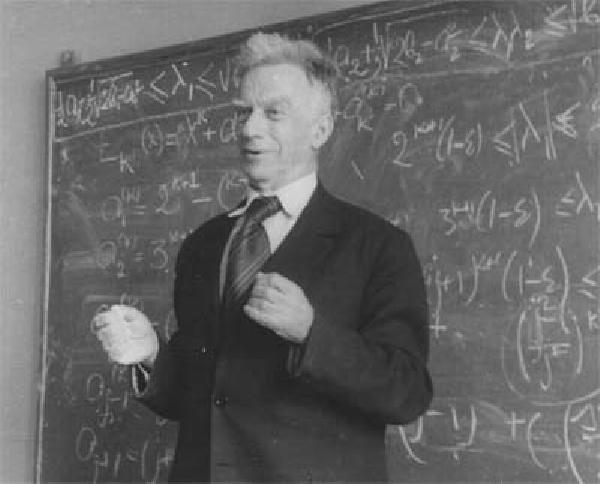
\includegraphics[scale=0.25]{Imagenes/Serguei_Sobolev.jpg}
\end{figure}
\end{frame}

\begin{frame}
\frametitle{Continuando la teoría}
De manera independientemente a finales de la década de 1940, el matemático francés, Laurent Schwartz (1915 - 2002) formalizó la teoría de distribuciones, \pause lo que le valió la Medalla Fields en 1950.
\end{frame}
\begin{frame}
\frametitle{Premio no recibido}
Que no recibió durante la entrega, ya que se le negó la visa para ingresar a los Estados Unidos.
\begin{figure}
    \centering
    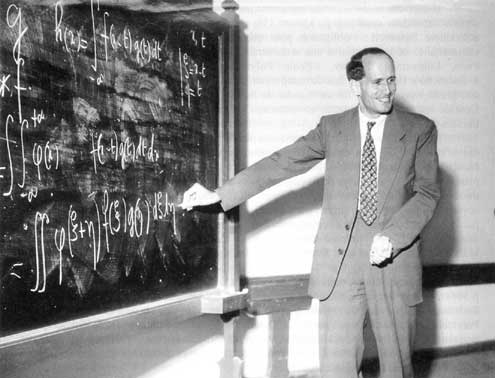
\includegraphics[scale=0.35]{Imagenes/Laurent_Schwartz.jpg}
\end{figure}
\end{frame}

\begin{frame}
\frametitle{Intención de la teoría}
Como el nombre lo sugiere, la teoría tiene como objetivo  \textocolor{cobalt}{extender la definición de una función}, \pause de manera tal que conceptos como el de la delta de Dirac $\delta (x)$ cuenten con una base matemática firme.
\end{frame}

\begin{frame}
\frametitle{Intención de la teoría}
En particular la teoría permite extender el concepto de derivada a todas las funciones localmente integrables y a entes aún más generales.
\end{frame}

\begin{frame}
\frametitle{Integrales de estudio}
Existen varias formas de presentar la teoría de distribuciones, se dará una breve introducción utilizando las integrales de secuencias de funciones del tipo:
\pause
\begin{equation}
\scaleint{6ex} f_{n} (x) \, g (x) \dd{x} \hspace{1cm} n = 1, 2, 3 , \ldots
\label{eq:ecuacion_1_99}
\end{equation}
\end{frame}

\begin{frame}
\frametitle{Conceptos importantes}
Para ello es necesario introducir tres conceptos:
\pause
\setbeamercolor{item projected}{bg=bananayellow,fg=ao}
\setbeamertemplate{enumerate items}{%
\usebeamercolor[bg]{item projected}%
\raisebox{1.5pt}{\colorbox{bg}{\color{fg}\footnotesize\insertenumlabel}}%
}
\begin{enumerate}[<+->]
\item El concepto de función de prueba.
\item El concepto de función admisible.
\item El concepto de convergencia débil.
\end{enumerate}
\end{frame}

\begin{frame}
\frametitle{Secuencia de funciones}
Hemos visto que una secuencia de funciones $f_{n} (x)$ tal como la secuencia delta de funciones, definida en \ref{secuencias_delta}, \pause nos lleva al concepto matemático de \enquote{función} delta, si la secuencia de integrales converge para funciones apropiadas $g (x)$.
\end{frame}

\begin{frame}
\frametitle{Pregunta interesante}
Pero \textocolor{carmine}{¿qué quiere decir que sean apropiadas?}
\pause
Si queremos definir conceptos tales como las \textbf{derivadas de la función delta}, entonces las funciones $g (x)$ deben ser diferenciables.
\end{frame}

\begin{frame}
\frametitle{Derivadas de las funciones}
Para definir las derivadas también hemos visto que al integrar por partes, para que las derivadas totales no contribuyan, es necesario que la función $g (x)$ tenga un comportamiento apropiado en infinito.
\end{frame}

\begin{frame}
\frametitle{Las funciones apropiadas}
Definimos entonces las funciones $g (x)$ como:
\pause
Decimos que las función $g (x)$ en la ec. (\ref{eq:ecuacion_1_99}), es una \textocolor{darkgreen}{función de prueba}, si es infinitamente diferenciable (clase $C^{\infty}$) y es idénticamente cero fuera de algún intervalo $(a, b)$ (en general este intervalo es diferente para funciones $g (x)$ diferentes).
\end{frame}

\begin{frame}
\frametitle{Las funciones de prueba}
El nombre de funciones de prueba es adecuado, dado que por ejemplo, \textocolor{alizarin}{la propiedad de filtro} de las secuencias delta, se prueba sobre estas funciones.
\end{frame}

\begin{frame}
\frametitle{Requerimiento de otras funciones}
Habiendo definido las funciones de prueba, podemos ahora definir las \textocolor{amethyst}{funciones admisibles} (de las cuales seleccionaremos las funciones $f_{n}( x)$) y la \textocolor{americanrose}{convergencia débil}.
\end{frame}

\begin{frame}
\frametitle{Funciones admisibles}
Decimos que las funciones $f_{n} (x)$ en la ec. (\ref{eq:ecuacion_1_99}) son \textocolor{antiquefuchsia}{funciones admisibles}, si son infinitamente diferenciables.
\\
\bigskip
\pause
Su comportamiento en infinito puede ser arbitrario.
\end{frame}

\begin{frame}
\frametitle{Convergencia débil}
Consideremos una secuencia de funciones admisibles $f_{n} (x)$ con $n = 1, 2, 3, \ldots$
\\
\bigskip
\pause
Decimos que esta secuencia es débilmente convergente si el límite:
\pause
\begin{equation}
\lim_{n \to \infty} \scaleint{6ex}_{\bs -\infty}^{\infty} f_{n}(x) \:  g (x) \, \dd{x}
\label{eq:ecuacion_1_100}
\end{equation}
existe para todas las funciones de prueba $g (x)$.
\end{frame}

\begin{frame}
\frametitle{Secuencias débilmente convergentes}
Una secuencia débilmente convergente puede o no puede converger en alguno de los sentidos de convergencia usual, como convergencia puntual.
\end{frame}

\begin{frame}
\frametitle{Concepto de distribución}
Podemos presentar ahora una definición rigurosa de una distribución de la siguiente manera:
\pause
Una \textocolor{auburn}{distribución} $\varphi (x)$ es un concepto matemático asociado con una secuencia débilmente convergente de funciones admisibles para la cual la integral simbólica:
\pause
\begin{equation}
\scaleint{6ex}_{\bs -\infty}^{\infty} \phi (x) \:  g (x) \, \dd{x}
\label{eq:ecuacion_1_101}
\end{equation}
\end{frame}

\begin{frame}
\frametitle{Significado de la distribución}
Tiene un significado preciso, por medio de la prescripción:
\pause
\begin{equation}
\scaleint{6ex}_{\bs -\infty}^{\infty} \phi (x) \: g (x) \, \dd{x} = \lim_{n \to \infty} f_{n} (x) \: g (x) \, \dd{x}
\label{eq:ecuacion_1_102}
\end{equation}
\end{frame}

\section{La delta de Dirac}
\frame[allowframebreaks]{\tableofcontents[currentsection, hideothersubsections]}
\subsection{Definición}

\begin{frame}
\frametitle{Expresando la delta de Dirac}
Informalmente la delta de Dirac es una \enquote{\textocolor{blue-violet}{función}} que representa un pico infinitamente agudo expresado simbólicamente por:
\pause
\begin{equation}
\delta (x) = \begin{cases}
0 & x \neq 0 \\
\infty & x = 0
\end{cases}
\label{eq:ecuacion_delta_01}
\end{equation}
\end{frame}

\begin{frame}
\frametitle{Integral normalizada}
Pero tal que la integral de $\delta (x)$ está normalizada a la unidad:
\pause
\begin{equation}
\scaleint{6ex}_{\bs -\infty}^{\infty} \delta (x) \: \dd{x} = 1 
\label{eq:ecuacion_delta_02}
\end{equation}
\end{frame}

\subsection{Propiedad de filtro}

\begin{frame}
\frametitle{Propiedades de la $\delta (x)$}
La delta de Dirac satisface la siguiente propiedad:
\pause
\begin{equation}
\scaleint{6ex}_{\bs -\infty}^{\infty} \delta (x) \: f (x) \: \dd{x} = f (0)
\label{eq:ecuacion_delta_03}
\end{equation}
donde $f (x)$ es una función continua.
\end{frame}

\begin{frame}
\frametitle{Resolviendo la integral}
Esta integral puede ser \enquote{\textocolor{red}{evaluada}} utilizando siguiente argumento: \pause
\setbeamercolor{item projected}{bg=bole,fg=white}
\setbeamertemplate{enumerate items}{%
\usebeamercolor[bg]{item projected}%
\raisebox{1.5pt}{\colorbox{bg}{\color{fg}\footnotesize\insertenumlabel}}%
}
\begin{enumerate}[<+->]
\item Dado que $\delta (x) = 0$ para $x \neq 0$.
\item Podemos cambiar los límites de integración en la ecuación (\ref{eq:ecuacion_delta_03}) a $- \epsilon$ y $+ \epsilon$, donde $\epsilon$ es un número positivo infinitesimal.
\seti
\end{enumerate}
\end{frame}

\begin{frame}
\frametitle{Resolviendo la integral}
\setbeamercolor{item projected}{bg=bole,fg=white}
\setbeamertemplate{enumerate items}{%
\usebeamercolor[bg]{item projected}%
\raisebox{1.5pt}{\colorbox{bg}{\color{fg}\footnotesize\insertenumlabel}}%
}
\begin{enumerate}[<+->]
\conti
\item Más aún, dado que $f (x)$ es continua en $x = 0$, sus valores dentro del intervalo $( - \epsilon, + \epsilon)$ no diferirán mucho de $f (0)$ y podemos hacer la siguiente aproximación:
\begin{eqnarray*}
\begin{aligned}
\scaleint{6ex}_{\bs -\infty}^{\infty} \delta (x) \: f (x) \: \dd{x} &= \scaleint{6ex}_{\bs -\epsilon}^{\epsilon} \delta (x) \: f (x) \: \dd{x} \\[0.5em] \pause
&\approx f (0) \scaleint{6ex}_{\bs -\infty}^{\infty} \delta (x) \: \dd{x}
\end{aligned}
\end{eqnarray*}
Esta aproximación mejora cuando $\epsilon \to 0$.
\end{enumerate}
\end{frame}

\begin{frame}
\frametitle{Consideración importante}
Pero:
\pause
\begin{align*}
\scaleint{6ex}_{\bs -\epsilon}^{+\epsilon} \delta (x) \: \dd{x} = 1
\end{align*}
para todos los valores de $\epsilon$, por que $\delta (x) = 0$ para $x \neq 0$ y $\delta (x)$ está normalizada.
\end{frame}

\begin{frame}
\frametitle{Tomando el límite}
Así en el límite $\epsilon \to 0$, se tiene:
\pause
\begin{align*}
\scaleint{6ex}_{\bs -\infty}^{\infty} \delta (x) \: f (x) \: \dd{x} = f (0)
\end{align*}
\textbf{Nota: } Los límites $-\infty$ y $+\infty$ se pueden reemplazar por cualesquiera números $a$ y $b$, tales que $a < 0 < b$.
\end{frame}

\begin{frame}
\frametitle{Propiedad de filtro}
Esta integral se le conoce también como \textocolor{bostonuniversityred}{propiedad de filtro} de la función delta, \pause ya que $\delta (x)$ actúa como un filtro, seleccionando de todos los posibles valores de $f (x)$ su valor en el punto $x = 0$.
\end{frame}

\subsection{Secuencias delta}\label{secuencias_delta}

\begin{frame}
\frametitle{Haciendo la referencia correcta}
La afirmación de que la función $\delta (x)$ está dada por la expresión (\ref{eq:ecuacion_delta_01}) \textit{\textocolor{brown(web)}{o es una afirmación apropiada y no se puede utilizar para definir una función}}, mucho menos para una función integrable.
\end{frame}

\begin{frame}
\frametitle{Referencia alterna}
Una posible definición alterna, podría ser el definir la función $\delta (x)$ como la función que satisface la propiedad de filtro (\ref{eq:ecuacion_delta_03}):
\pause
\begin{align*}
\scaleint{6ex}_{\bs -\infty}^{+ \infty} \delta (x) \: f (x) \: \dd{x} = f (0)
\end{align*}
para toda función continua $f (x)$. 
\end{frame}

\begin{frame}
\frametitle{Complicación matemática}
Sin embargo es posible demostrar que no existe ninguna función con esa propiedad.
\\
\bigskip
\pause
Por lo que:
\pause
\begin{center}
\textit{¡¡la función delta no es una función en el sentido matemático usual!!}
\end{center}
\end{frame}

\begin{frame}
\frametitle{Respondiendo al problema}
¿Qué se hace entonces? \pause ¿Dirac nos engañó con su propuesta?
\\
\bigskip
\pause
Lo que sucede es que existen secuencias de funciones de pico pronunciado, las cuales en el límite en que el pico es infinitamente delgado e infinitamente alto, satisfacen la propiedad de filtro.
\end{frame}

\begin{frame}
\frametitle{Proponiendo una secuencia}
La siguiente puede ser una secuencia $\phi_{n} (x)$ con $n = 1, 2, 3, \ldots$, tal que:
\pause
\begin{align*}
\lim_{n \to \infty} \scaleint{6ex}_{\bs -\infty}^{+ \infty} \phi_{n} (x) \: f (x) \dd{x} =  f (0)
\end{align*}
\end{frame}

\begin{frame}
\frametitle{Definiendo la secuencia delta}
Llamamos secuencias delta $\delta_{n} (x)$ a una secuencia de funciones de pico pronunciado, que satisfacen:
\pause
\begin{align*}
\lim_{n \to \infty} \scaleint{6ex}_{\bs -\infty}^{+ \infty} \phi_{n} (x) \: f (x) \: \dd{x} =  f (0)
\end{align*}
\end{frame}

\begin{frame}
\frametitle{Ejemplo de una secuencia}
La secuencia de funciones:
\pause
\begin{equation}
\phi_{n} (x) = \begin{cases}
0 & x < - \dfrac{1}{2 \, n} \\
n & - \dfrac{1}{2 \, n} < x < \dfrac{1}{2 \, n} \\
0 & 0 >  \dfrac{1}{2 \, n}
\end{cases}
\hspace{1cm} n = 1, 2, 3, \ldots
\label{eq:ecuacion_delta_04}
\end{equation}
es una secuencia delta.
\end{frame}

\begin{frame}
\frametitle{Graficando la secuencia}
\begin{figure}[H]
    \centering
    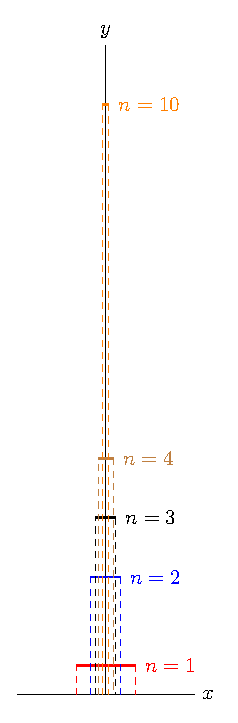
\includegraphics[scale=0.5]{Imagenes/plot_secuencia_delta.eps}
    \caption{Secuencia delta para valores de $n = 1, 2, \ldots, 10$. El área debajo de la curva para cada $\phi_{n}$ siempre es $1$.}
    \label{fig:secuncia_delta_01}
\end{figure}
\end{frame}

\begin{frame}
\frametitle{Demostración}
Para verificar esta afirmación consideremos la integral:
\pause
%Apuntes FETI página 46
\begin{align*}
\scaleint{6ex}_{\bs -\infty}^{\infty} \phi_{n} (x) \: f (x) \dd{x}
\end{align*}
para cualquier función continua arbitraria $f (x)$.
\end{frame}

\begin{frame}
\frametitle{Demostración}
De la expresión (\ref{eq:ecuacion_delta_04}) para la secuencia delta se tiene:
\pause
\begin{eqnarray*}
\scaleint{6ex}_{\bs -\infty}^{+ \infty} \phi_{n} (x) \: f (x) \dd{x} &=  \pause \scaleint{6ex}_{\bs -\frac{1}{2 \, n}}^{\frac{1}{2 \, n}} n \: f (x) \: \dd{x} = \\[0.5em] \pause
&= n \scaleint{6ex}_{\bs -\frac{1}{2 \, n}}^{\frac{1}{2 \, n}} f (x) \:  \dd{x}
\end{eqnarray*}
\end{frame}

\begin{frame}
\frametitle{Apoyo del cálculo}
Utilizando el teorema del valor medio para integrales, podemos deducir que:
\pause
\begin{eqnarray*}
\begin{aligned}
n \, \scaleint{6ex}_{\bs -\frac{1}{2 \, n}}^{\frac{1}{2 \, n}} f (x) \dd{x} \pause &= n \: \dfrac{1}{n} f (\xi) = \\[0.5em] \pause
&= f (\xi), \hspace{1cm} - \dfrac{1}{2 \, n} \leq \xi \leq \dfrac{1}{2 \, n}
\end{aligned}
\end{eqnarray*}
En el límite cuando $n \to \infty$, $\xi \to 0$.
\end{frame}

\begin{frame}
\frametitle{Usando la continuidad de la función}
De la continuidad de la función $f (x)$ se sigue que $f (\xi) \to f (0)$, obteniendo así el resultado:
\pause
\begin{align*}
\lim_{n \to \infty} \scaleint{6ex}_{\bs -\infty}^{+ \infty} \: \phi_{n} (x) \: f (x) \: \dd{x} = f (0)
\end{align*}
lo que nos dice que la secuencia (\ref{eq:ecuacion_delta_04}), es una secuencia delta. \pause  Nótese que la secuencia delta (\ref{eq:ecuacion_delta_04}) no es derivable en el punto $x = 0$.
\end{frame}

\begin{frame}
\frametitle{Secuencias atractivas y de utilidad}
Para muchos propósitos es deseable construir secuencias delta de funciones que sean continuas y diferenciables.
\\
\bigskip
\pause 
Por ejemplo, en las figuras (\ref{fig:plot_secuencia_01}), (\ref{fig:plot_secuencia_02}) y (\ref{fig:plot_secuencia_03}) podemos apreciar algunas secuencias delta con estas características:
\end{frame}

\begin{frame}
\frametitle{Una secuencia delta}
\begin{figure}[H]
    \centering
    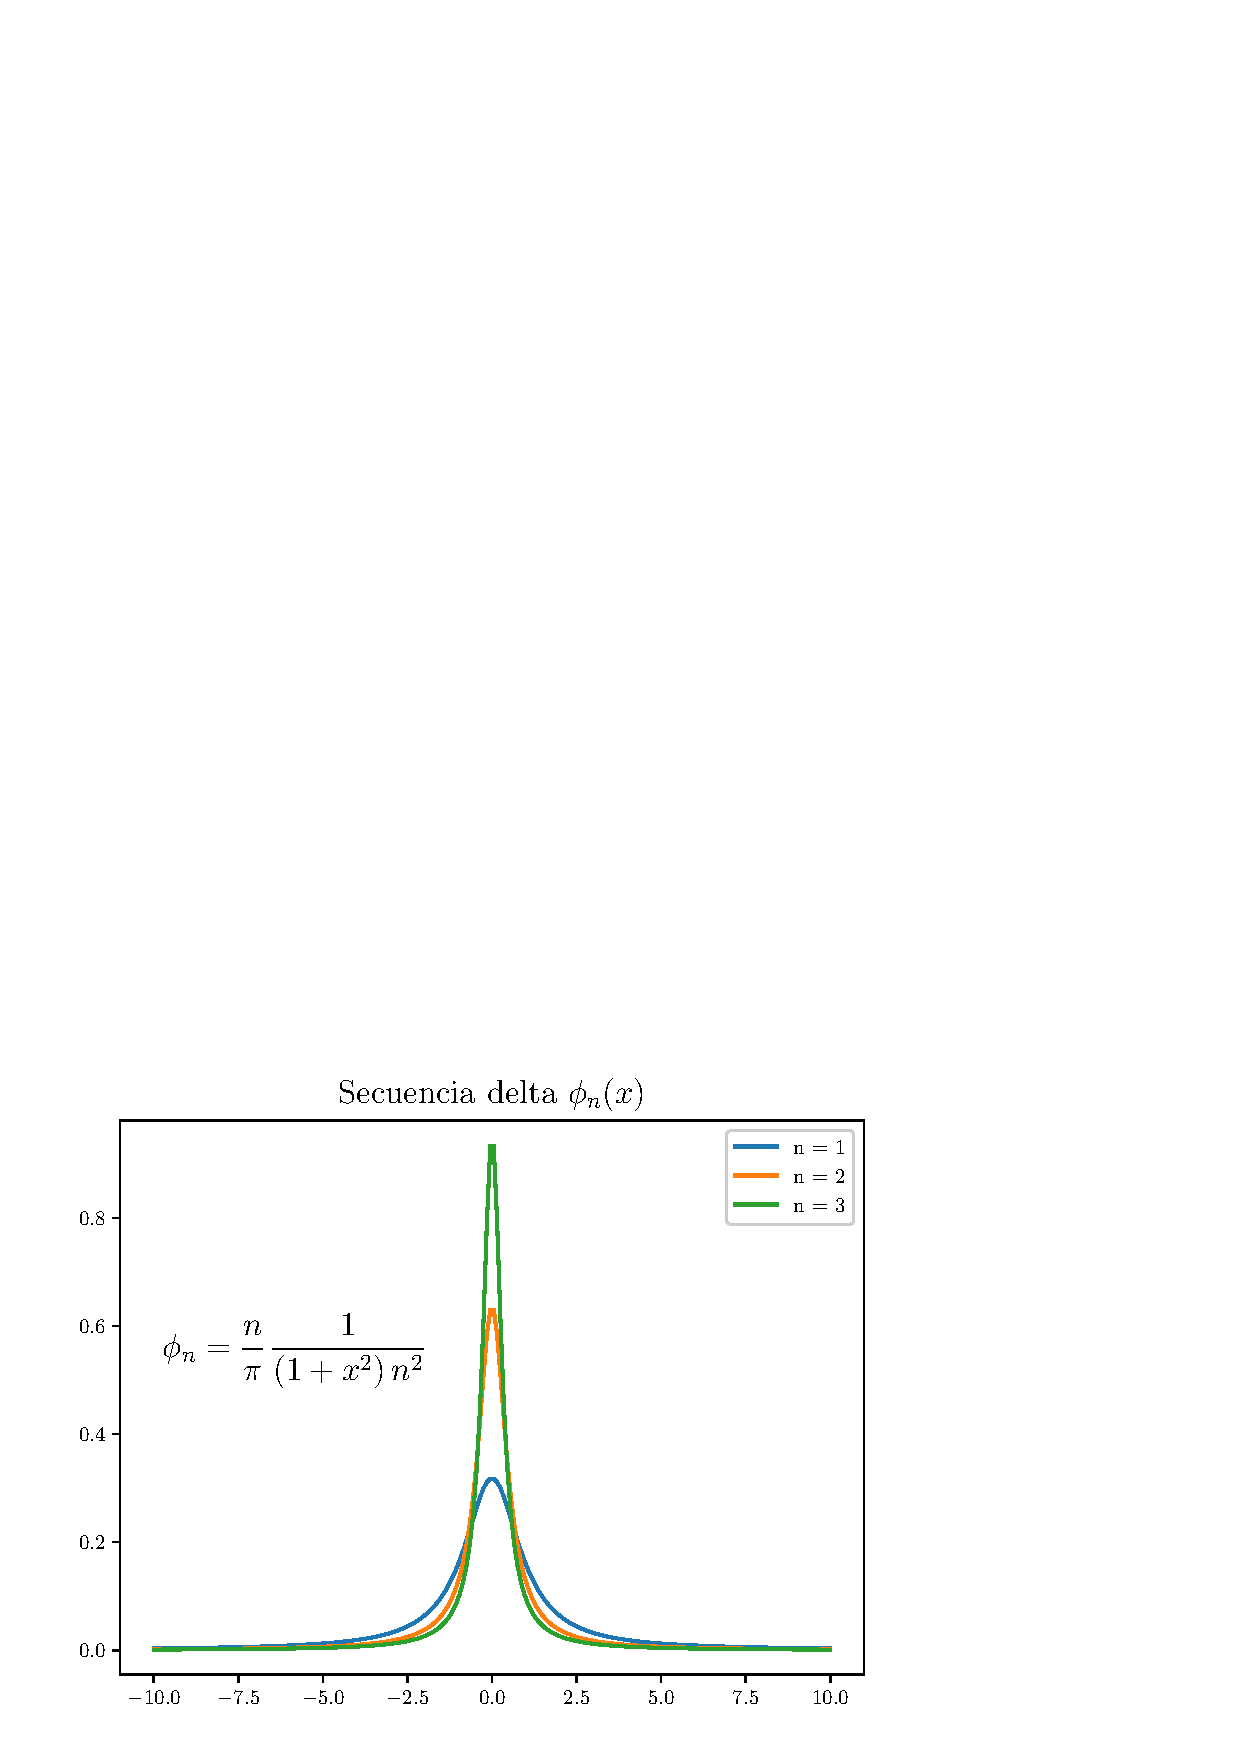
\includegraphics[scale=0.7]{Imagenes/secuencia_delta_01.pdf}
    %\caption{Secuencia para $\phi_{n}$ con $n=1,2,3$}
    \label{fig:plot_secuencia_01}
\end{figure}
\end{frame}

\begin{frame}
\frametitle{Otra secuencia delta}
\begin{figure}[H]
    \centering
    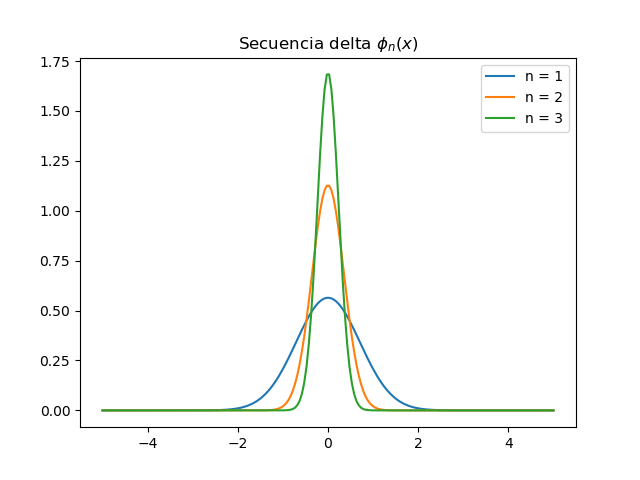
\includegraphics[scale=0.7]{Imagenes/secuencia_delta_02.pdf}
    %\caption{Secuencia para $\phi_{n}$ con una función exponencial.}
    \label{fig:plot_secuencia_02}
\end{figure}
\end{frame}

\begin{frame}
\frametitle{Una secuencia delta más}
\begin{figure}[H]
    \centering
    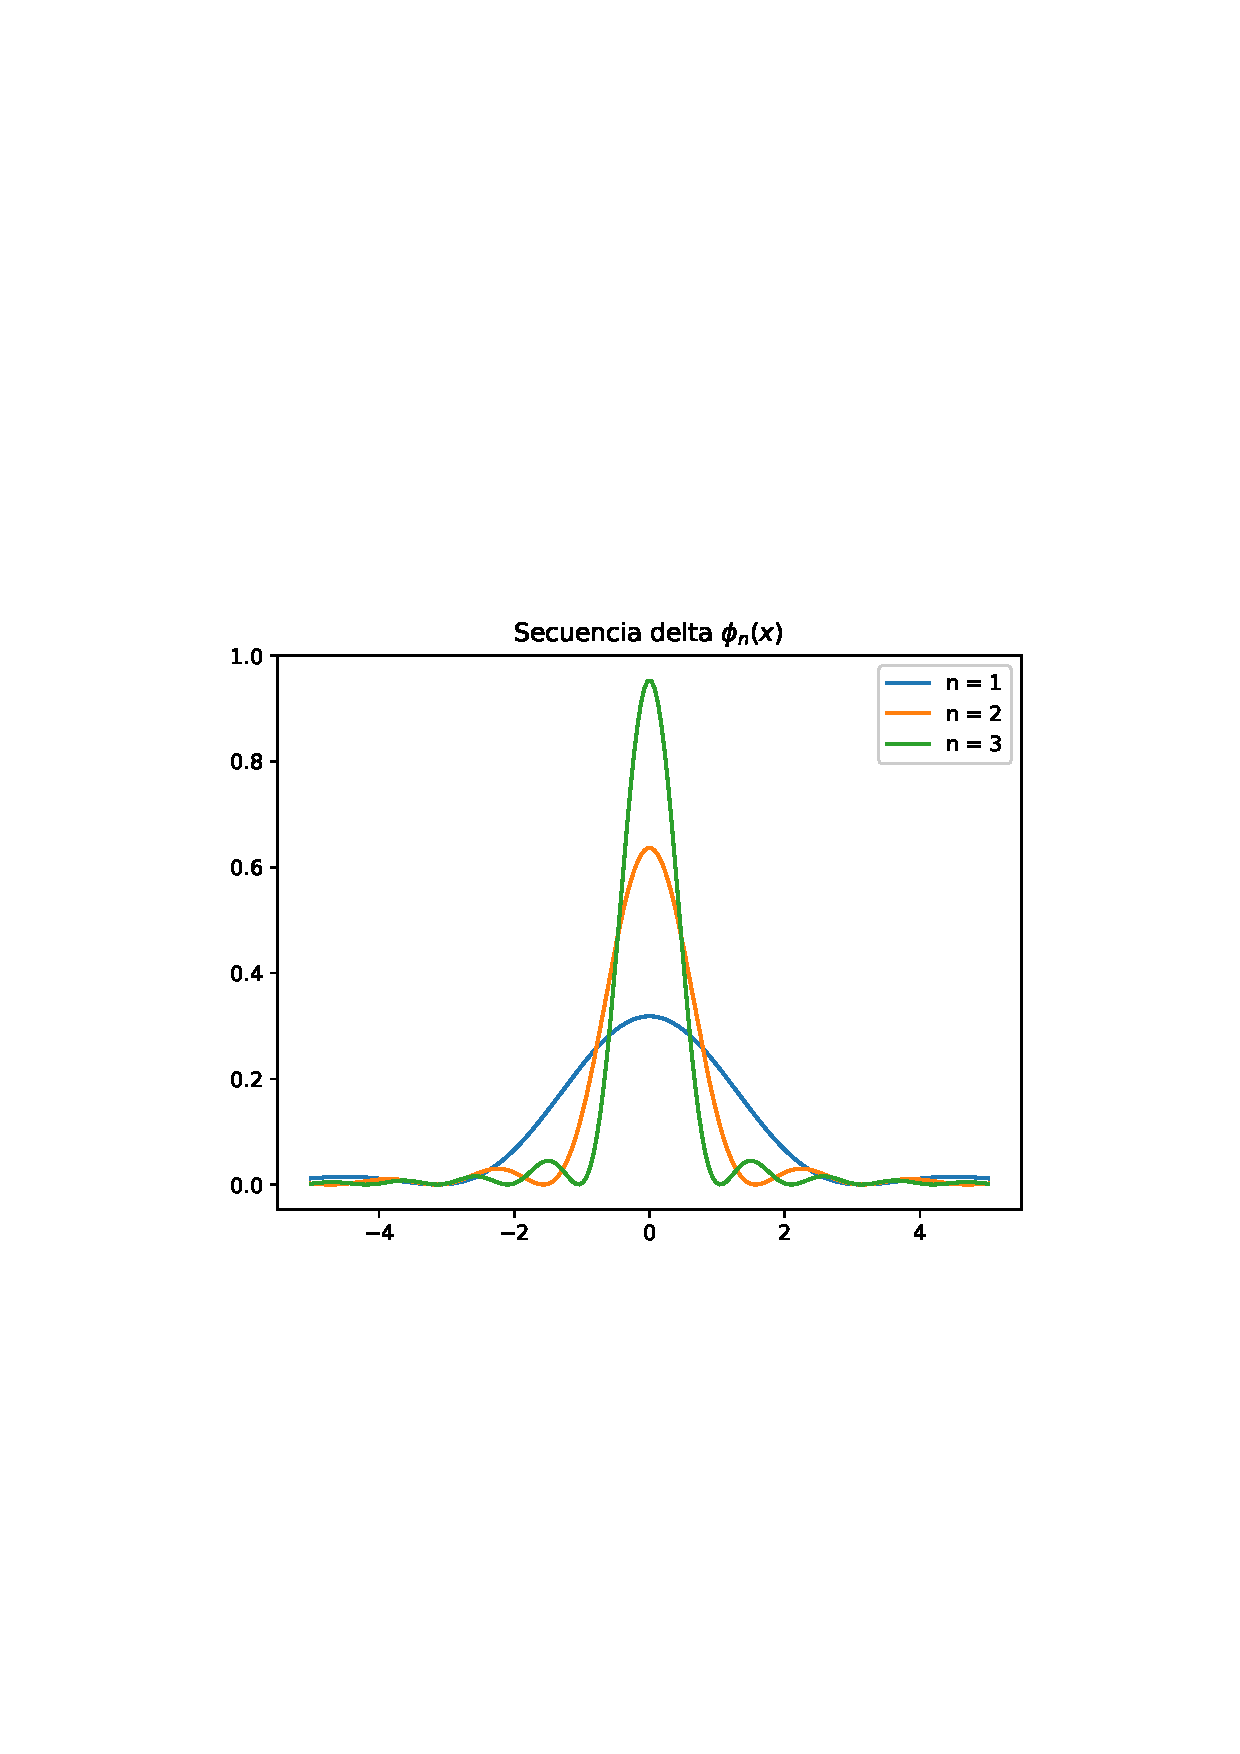
\includegraphics[scale=0.7]{Imagenes/secuencia_delta_03.pdf}
    %\caption{Secuencia para $\phi_{n}$ con una función $\sin^{2}(x)/x$}
    \label{fig:plot_secuencia_03}
\end{figure}
\end{frame}

\begin{frame}
\frametitle{Consideración relevante}
Tomemos en cuenta que no es correcto expresar que éstas secuencias convergen a la función delta: \pause los límites de esas secuencias \textocolor{burgundy}{no existen}, de acuerdo a las definiciones conocidas de convergencia.
\end{frame}

\begin{frame}
\frametitle{Secuencias normalizadas}
Todas estas funciones están normalizadas a la unidad:
\pause
\begin{equation}
\lim_{n \to \infty} \scaleint{6ex}_{\bs - \infty}^{+ \infty} \phi_{n} (x) \: \dd{x} = 1
\label{eq:ecuacion_delta_05}
\end{equation}
\end{frame}

\subsection{Propiedades de la delta de Dirac}

\begin{frame}
\frametitle{Manejando la delta de Dirac}
Una vez que hemos definido la delta de Dirac, nos gustaría saber ahora como operar con y en ella. 
\\
\bigskip
\pause
¿Es posible decir algo sobre su derivada? \pause La respuesta a esta pregunta es afirmativa y las secuencias delta hechas de funciones diferenciables nos permiten responder a la pregunta de manera precisa.
\end{frame}

\begin{frame}
\frametitle{Diferenciando la secuencia delta}
Por ejemplo, sea la secuencia delta:
\pause
\begin{align*}
\phi_{n} &= \dfrac{n}{\sqrt{\pi}} e^{-n^{2} x^{2}}
\end{align*}
\pause
entonces, al diferenciar la secuencia:
\pause
\begin{align*}
\dv{\phi_{n}(x)}{x} = - \dfrac{2 \: n^{3}}{\sqrt{\pi}} \: x \: \exp(-n^{2} \: x^{2})
\end{align*}
\end{frame}

\begin{frame}
\frametitle{Gráfica de la derivada de la secuencia}
\begin{figure}[H]
    \centering
    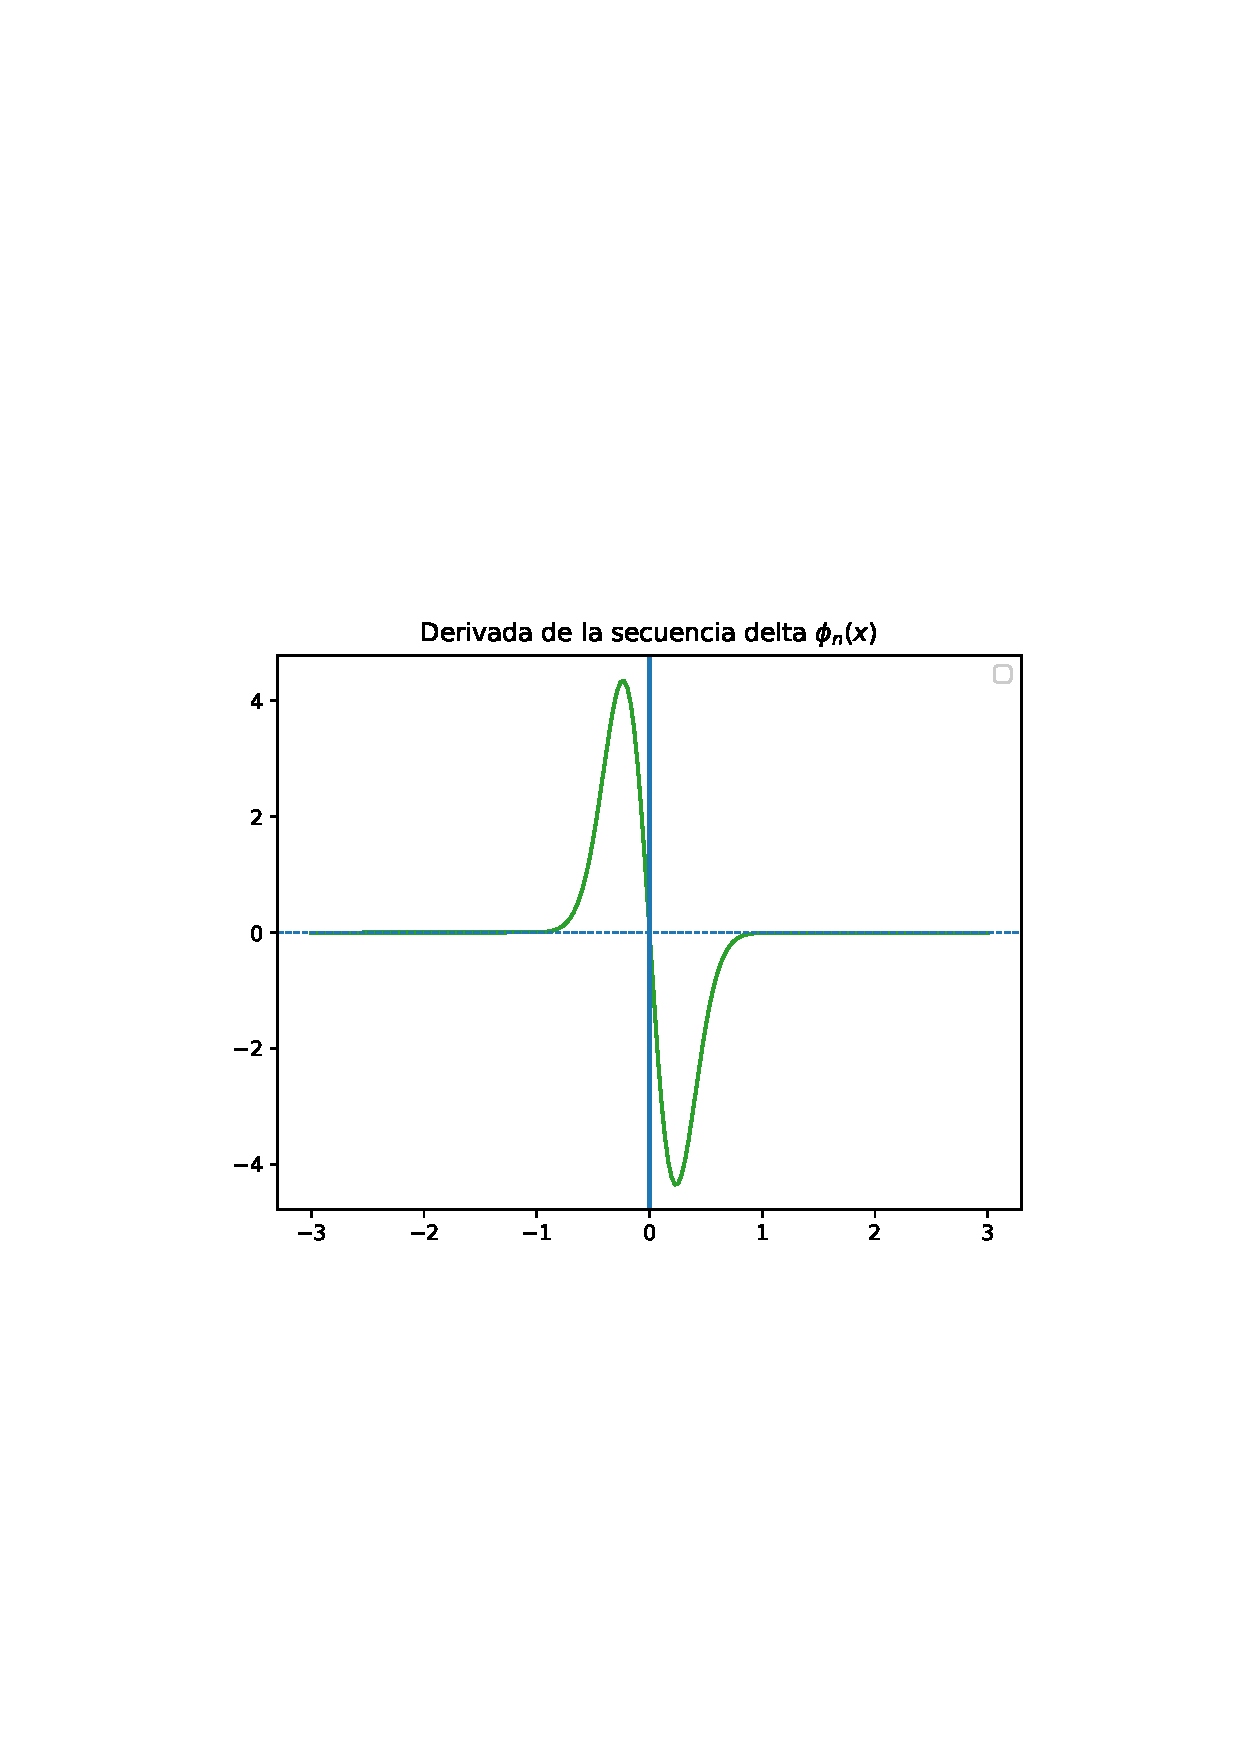
\includegraphics[scale=0.8]{Imagenes/secuencia_delta_04.pdf}
    % \caption{Derivada de la secuencia delta.}
    \label{fig:fig_figura_delta_04}
\end{figure}
\end{frame}

\begin{frame}
\frametitle{Usando una integral}
Consideremos ahora la integral:
\begin{align*}
\scaleint{6ex}_{\bs -\infty}^{+\infty} \dv{\phi_{n}(x)}{x} \: f (x) \dd{x}
\end{align*}
donde $f (x)$ es diferenciable.
\\
\bigskip
\pause
Integrando por partes, se obtiene:
\pause
\begin{align*}
\scaleint{6ex}_{\bs -\infty}^{+\infty} \dv{\phi_{n}(x)}{x} \: f (x) \dd{x} = \phi_{n} \: f (x) \eval_{-\infty}^{+\infty} - \scaleint{6ex}_{\bs -\infty}^{+\infty} \phi_{n} \: \dv{f (x)}{x} \dd{x}
\end{align*}
\end{frame}

\begin{frame}
\frametitle{Resolviendo la integral}
Suponemos que:
\pause
\begin{align*}
\lim_{n \to \infty} \left( \dfrac{n}{\sqrt{\pi}} \right) \exp(-n^{2} \: x^{2}) \: f (x) = 0
\end{align*}
\pause
Esto normalmente es cierto, ya que estamos considerando funciones para las cuales la integral:
\pause
\begin{align*}
\scaleint{6ex}_{\bs -\infty}^{+\infty} \phi_{n}(x) \: f (x) \dd{x} 
\end{align*}
converge.
\end{frame}

\begin{frame}
\frametitle{Resolviendo la integral}
Entonces, haciendo que $n \to \infty$, tenemos:
\pause
\begin{eqnarray*}
\begin{aligned}
\lim_{n \to \infty} \scaleint{6ex}_{\bs -\infty}^{+\infty} \dv{\phi_{n}(x)}{x} \: f (x) \dd{x} &= - \lim_{n \to \infty} \phi_{n}(x) \: \pderivada{f} (x) \dd{x} =  \\[0.5em] \pause
&= - \pderivada{f} (0)
\end{aligned}
\end{eqnarray*}
\pause
Vemos entonces que la secuencia $\pderivada{\phi} (x)$ está relacionada con la propiedad de filtro.
\end{frame}

\begin{frame}
\frametitle{Propiedad de filtro para las derivadas}
La delta de Dirac satisface la siguiente propiedad:
\pause
\begin{align*}
\scaleint{6ex}_{\bs -\infty}^{+\infty} \dv{\delta(x)}{x} \: f (x) \: \dd{x} = - \dv{f (0)}{x}
\end{align*}
con $f (x)$ una función diferenciable.
\end{frame}

\begin{frame}
\frametitle{Propiedad para las derivadas de orden superior}
Con la idea anterior, se presenta la propiedad para las derivadas de orden superior de $\delta (x)$:
\pause
\begin{align*}
\scaleint{6ex}_{\bs -\infty}^{+\infty} \dv[m]{\delta (x)}{x} \: f (x) \dd{x} =  (-1)^{m} \: \dv[m]{f (0)}{x}
\end{align*}
\end{frame}

\begin{frame}
\frametitle{Casos en los que se cumple}
Es necesario enfatizar que la expresión anterior tiene significado sólo cuando asumimos directamente que las funciones involucradas son $m$ veces diferenciables y que las integrales:
\pause
\begin{align*}
\scaleint{6ex}_{\bs -\infty}^{+\infty} \dv[k]{\phi_{n}(x)}{x} \: f (x) \dd{x}
\end{align*}
convergen para todo valor de $n$ y para todo valor de $k$ de $0$ a $m$.
\end{frame}

\begin{frame}
\frametitle{Propiedades de la delta de Dirac}
La delta de Dirac satisface varias propiedades y conocerlas es de mucha utilidad cuando resolvemos problemas específicos en física. 
\end{frame}

\section{Propiedades de \texorpdfstring{$\delta (x)$}{d (x)}}
\frame{\tableofcontents[currentsection, hideothersubsections]}
\subsection{Lista de propiedades}

\begin{frame}
\frametitle{Revisando las propiedades}
La siguiente lista contiene propiedades que se pueden demostrar directamente de la definición:
\pause
\setbeamercolor{item projected}{bg=cadet,fg=white}
\setbeamertemplate{enumerate items}{%
\usebeamercolor[bg]{item projected}%
\raisebox{1.5pt}{\colorbox{bg}{\color{fg}\footnotesize\insertenumlabel}}%
}
\begin{enumerate}[<+->]
\item $\delta (x) f (x) = f (0) \, \delta (x)$
\item $\delta (-x) = \delta (x)$
\item $\pderivada{\delta} (- x) = - \pderivada{\delta} (x)$
\item $\delta(a \, x) = \dfrac{1}{\abs{a}} \: \delta (x), \hspace{1cm} a \neq 0$
\item $\delta (x^{2} - a^{2}) = \dfrac{1}{2 \, a} \left[ \delta (x + a) + \delta (x - a) \right] \hspace{1cm} a > 0$
\seti
\end{enumerate}
\end{frame}

\begin{frame}
\frametitle{Revisando las propiedades}
\setbeamercolor{item projected}{bg=cadet,fg=white}
\setbeamertemplate{enumerate items}{%
\usebeamercolor[bg]{item projected}%
\raisebox{1.5pt}{\colorbox{bg}{\color{fg}\footnotesize\insertenumlabel}}%
}
\begin{enumerate}[<+->]
\conti
\item $x \: \delta(x) = 0$
\item $f (x) \: \delta(x - a) = f(a) \: \delta(x - a)$
\item $\delta (x - \pderivada{x}) = 0 \hspace{1cm} x \neq \pderivada{x}$
\item $\delta (x - \pderivada{x}) = \delta (\pderivada{x} - x)$
\seti
\end{enumerate}
\end{frame}

\begin{frame}
\frametitle{Revisando las propiedades}
\setbeamercolor{item projected}{bg=cadet,fg=white}
\setbeamertemplate{enumerate items}{%
\usebeamercolor[bg]{item projected}%
\raisebox{1.5pt}{\colorbox{bg}{\color{fg}\footnotesize\insertenumlabel}}%
}
\begin{enumerate}[<+->]
\conti
\item $\scaleint{6ex}_{\bs -\infty}^{\infty} \delta (x) \, f (x) \dd{x} = f (0)$
\item $\scaleint{6ex}_{\bs -\infty}^{\infty} \pderivada{\delta} (x) \, f (x) \dd{x} = - \pderivada{f} (0)$
\item $\scaleint{6ex}_{\bs a}^{b} \delta (x - \pderivada{x}) \dd{\pderivada{x}} = 1 \hspace{1cm} a < x < b$
\item $\scaleint{6ex}_{\bs -\infty}^{\infty} \delta (x - \pderivada{x}) \, f (\pderivada{x}) \dd{\pderivada{x}} = f (x)$
\seti
\end{enumerate}
\end{frame}

\begin{frame}
\frametitle{Revisando las propiedades}
\setbeamercolor{item projected}{bg=cadet,fg=white}
\setbeamertemplate{enumerate items}{%
\usebeamercolor[bg]{item projected}%
\raisebox{1.5pt}{\colorbox{bg}{\color{fg}\footnotesize\insertenumlabel}}%
}
\begin{enumerate}[<+->]
\conti
\item $\scaleint{6ex}_{\bs -\infty}^{\infty} \delta (\sderivada{x} - \pderivada{x}) \, \delta (\sderivada{x} - x) \dd{\sderivada{x}} = (\pderivada{x} - x)$
\item $\scaleint{6ex}_{\bs -\infty}^{\infty} f (x) \: \delta (x - a) \: \dd{x} = f(a)$
\item $\scaleint{6ex} \delta (a - x) \: \delta (x - b) \: \dd{x} = \delta (a - b)$
\seti
\end{enumerate}
\end{frame}

\begin{frame}
\frametitle{Revisando las propiedades}
\setbeamercolor{item projected}{bg=cadet,fg=white}
\setbeamertemplate{enumerate items}{%
\usebeamercolor[bg]{item projected}%
\raisebox{1.5pt}{\colorbox{bg}{\color{fg}\footnotesize\insertenumlabel}}%
}
\begin{enumerate}[<+->]
\conti
\item Si la función $g (x)$ tiene una raíz o cero en $x_{0}$:
\begin{align*}
\delta ( g (x) ) = \nsum_{i=1}^{N} \dfrac{\delta (x - x_{i})}{\abs{\pderivada{g} (x_{i})}}
\end{align*}
donde los $x_{i}$ son los ceros simples de $f (x)$.
\end{enumerate}
\end{frame}

\section{Introduciendo más variables}
\frame{\tableofcontents[currentsection, hideothersubsections]}
\subsection{Expandiendo la delta de Dirac}

\begin{frame}
\frametitle{Ampliando la función}
Al introducir más variables:
\pause
\begin{equation}
\delta (\va{\bm{r}} - \va{\bm{r_{0}}}) = \delta (x - x_{0}) \: \delta (y - y_{0}) \: \delta (z - z_{0})
\label{eq:ecuacion_A_03}
\end{equation}
\pause
de manera que al integrar sobre todo el espacio tenemos:
\pause
\begin{align*}
\scaleint{6ex} \delta (\va{\bm{r}} - \va{\bm{r_{0}}}) \: \dd{x} \dd{y}  \dd{z} = 1
\end{align*}
\end{frame}

\begin{frame}
\frametitle{Usando la $\delta (x)$}
La función delta permite especificar la densidad de carga debida a un conjunto de $N$ cargas puntuales de valores $q_{i}$ situadas en posiciones $\va{r_{i}}$ como:
\pause
\begin{equation}
\rho (\va{r}) = \sum_{i=1}^{N} q_{i} \: \delta(\va{r} - \va{r_{i}})
\label{eq:ecuacion_A_04}
\end{equation}
\end{frame}

\begin{frame}
\frametitle{Recuperando el potencial}
Las propiedades de la función delta permiten obtener el potencial $\varphi(\va{r})$ evaluando la función dentro de la integral en los puntos $\va{r_{i}}$, es decir:
\pause
\begin{eqnarray}
\begin{aligned}[b]
\varphi(\va{r}) &= \pause \scaleint{6ex} \dfrac{\rho(\va{\pderivada{r}})}{\abs{\va{r} - \va{\pderivada{r}}}} \: d^{3} \pderivada{r} = \pause \nsum_{i=1}^{N} q_{i} \scaleint{6ex} \dfrac{\delta ( \va{r} - \va{r_{i}})}{\abs{ \va{r} - \va{\pderivada{r}} }} \: d^{3} \pderivada{r} = \\[0.5em] \pause
&= \nsum_{i=1}^{N} \dfrac{q_{i}}{\abs{ \va{r} - \va{r_{i}} }}
\end{aligned}
\label{eq:ecuacion_A_05}
\end{eqnarray}
\pause
Nótese que $\delta (x)$ tiene unidades de inverso de $x$ y $\delta (\va{r})$ tiene unidades de densidad numérica.
\end{frame}

\begin{frame}
\frametitle{Cambiando las coordenadas}
La función $\delta (x)$ toma una forma particular en coordenadas cilíndricas y esféricas, dadas por la condición de normalización:
\pause
\setbeamercolor{item projected}{bg=byzantium,fg=white}
\setbeamertemplate{enumerate items}{%
\usebeamercolor[bg]{item projected}%
\raisebox{1.5pt}{\colorbox{bg}{\color{fg}\footnotesize\insertenumlabel}}%
}
\begin{enumerate}[<+->]
\item Para coordenadas cilíndricas:
\begin{eqnarray*}
\begin{aligned}
&\scaleint{6ex} \delta (\va{r} - \va{r}_{0}) \: R \: \dd{R} \: \dd{\varphi} \: \dd{z} \\[0.5em] \pause 
&\Rightarrow \delta (\va{r}) =  \dfrac{1}{R} \: \delta (R - R_{0}) \: \delta (\varphi - \varphi_{0}) \: \delta (z - z_{0})
\end{aligned}
\end{eqnarray*}
\seti
\end{enumerate}
\end{frame}

\begin{frame}
\frametitle{Cambiando las coordenadas}
\setbeamercolor{item projected}{bg=byzantium,fg=white}
\setbeamertemplate{enumerate items}{%
\usebeamercolor[bg]{item projected}%
\raisebox{1.5pt}{\colorbox{bg}{\color{fg}\footnotesize\insertenumlabel}}%
}
\begin{enumerate}[<+->]
\conti
\item Para coordenadas esféricas:
\begin{eqnarray*}
\begin{aligned}
\scaleint{6ex} & \delta (\va{r} - \va{r}_{0}) \: r^{2} \, \dd{r} \, \sin \theta \, \dd{\theta} \, \dd{\varphi} = 1 \\[0.5em] \pause
&\Rightarrow \delta (\va{r}) = \dfrac{1}{r^{2}} \: \delta (r - r_{0}) \, \delta (\cos \theta - \cos \theta_{0}) \, \delta (\varphi - \varphi_{0})
\end{aligned}
\end{eqnarray*}
\end{enumerate}
\end{frame}

\begin{frame}
\frametitle{Algunas funciones al límite}
Algunas funciones que en el límite generan la función delta:
\pause
\begin{eqnarray*}
\begin{aligned}
\delta(x) = \begin{cases}
\displaystyle
\lim_{\varepsilon \to 0^{+}} \dfrac{1}{\pi} \, \dfrac{\varepsilon}{x^{2} + \varepsilon^{2}} & \mbox{Lorentz} \\[1em] \pause 
\displaystyle
\lim_{\sigma \to 0^{+}} \dfrac{1}{\sigma \, \sqrt{2 \, \pi}} \, \exp \left( - \dfrac{x^{2}}{2 \, \sigma^{2}} \right) & \mbox{Gaussiana} \\[1em] \pause
\displaystyle \lim_{\varepsilon \to 0^{+}} \dfrac{\sin(x / \varepsilon)}{ \pi \, x} & \mbox{Dirichlet} \\[1em] \pause
\displaystyle \lim_{L \to \infty} \dfrac{1}{2 \, \pi} \scaleint{6ex}_{\bs - \abs{L}}^{\abs{L}} \exp(i \, k \, x) \dd{k} & \mbox{Fourier}
\end{cases}
\end{aligned}
\end{eqnarray*}
\end{frame}

\section{Ejercicios}
\frame[allowframebreaks]{\tableofcontents[currentsection, hideothersubsections]}
\subsection{Calculando integrales}

\begin{frame}
\frametitle{Enunciado del Ejercicio 1}
Evalúa las siguientes integrales:
\pause
\begin{align*}
\scaleint{6ex}_{\bs -\infty}^{+\infty} (t^{2} + 3 t + 5) \delta (t) \dd{t}
\end{align*}
\pause
Nos apoyaremos con las propiedades que hemos enlistado.
\end{frame}

\begin{frame}
\frametitle{Resolviendo la integral}
Usando la propiedad de distribución de la integral, se tiene que:
\pause
\begin{eqnarray*}
\begin{aligned}
&\scaleint{6ex}_{\bs -\infty}^{+\infty} (t^{2} + 3 t + 5) \delta (t) \dd{t} = \\[0.5em] \pause
&= \scaleint{6ex}_{\bs -\infty}^{+\infty} t^{2} \delta (t) \dd{t} + \scaleint{6ex}_{\bs -\infty}^{+\infty} 3 t \delta (t) \dd{t} + \scaleint{6ex}_{\bs -\infty}^{+\infty} 5 \delta (t) \dd{t}
\end{aligned}
\end{eqnarray*}
\end{frame}

\begin{frame}
\frametitle{Usando una propiedad}
Ahora ocupamos la siguiente propiedad:
\pause
\begin{align*}
\scaleint{6ex}_{\bs -\infty}^{\infty} \delta (x) \, f (x) \dd{x} = f (0)
\end{align*}
\pause
Por lo que:
\begin{eqnarray*}
\begin{aligned}
\scaleint{6ex}_{\bs -\infty}^{+\infty} t^{2} \delta (t) \dd{t} = \pause 0 \\[0.5em] \pause
\scaleint{6ex}_{\bs -\infty}^{+\infty} 3 t \delta (t) \dd{t} =  \pause 0
\end{aligned}
\end{eqnarray*}
\end{frame}

\begin{frame}
\frametitle{Usando otra propiedad}
Entonces para la última integral, ocupamos la propiedad:
\pause
\begin{align*}
\scaleint{6ex}_{\bs -\infty}^{+\infty} \delta (t) \dd{t} =  1
\end{align*}
\pause
Llegando entonces al resultado:
\begin{eqnarray*}
\begin{aligned}
\scaleint{6ex}_{\bs -\infty}^{+\infty} 5 \, \delta (t) \dd{t} &= \pause 5 \scaleint{6ex}_{\bs -\infty}^{+\infty} \delta (t) \dd{t} = \\[0.5em] \pause
&= 5 \qed
\end{aligned}
\end{eqnarray*}
\end{frame}

\begin{frame}
\frametitle{Enunciado del Ejercicio 2}
Evalúa la siguiente integral:
\pause
\begin{align*}
\scaleint{6ex}_{\bs -\infty}^{+\infty} \dfrac{\cos (x) \, \delta (t)}{2 \exp(x) + 1}  \dd{t}
\end{align*}
\end{frame}

\begin{frame}
\frametitle{Resolviendo la integral}
Expresamos la integral como:
\pause
\begin{eqnarray*}
\begin{aligned}
\scaleint{6ex}_{\bs -\infty}^{+\infty} \dfrac{\cos (x) \, \delta (t)}{2 \exp(x) + 1} \dd{t} = \pause  
\scaleint{6ex}_{\bs -\infty}^{+\infty} \dfrac{\cos (x)}{2 \exp(x) + 1} \, \delta (t) \dd{t}
\end{aligned}
\end{eqnarray*}
\pause
Usamos la propiedad anterior:
\begin{align*}
\scaleint{6ex}_{\bs -\infty}^{\infty} \delta (x) \, f (x) \dd{x} = f (0)
\end{align*}
\end{frame}

\begin{frame}
\frametitle{Resultado}
Llegando entonces a lo siguiente:
\pause
\begin{eqnarray*}
\begin{aligned}
\scaleint{6ex}_{\bs -\infty}^{+\infty} \dfrac{\cos (x)}{2 \exp(x) + 1} \, \delta (t) \dd{t} &= \pause \dfrac{\cos (0)}{2 \exp (0) + 1} = \\[0.5em] \pause
&= \dfrac{1}{3} \qed
\end{aligned}
\end{eqnarray*}
\end{frame}

\begin{frame}
\frametitle{Ejercicio 3}
Evalúa la siguiente integral:
\pause
\begin{align*}
\scaleint{6ex}_{\bs -\infty}^{\infty} \sinh (2 t) \, \delta (2 - t) \dd{t}
\end{align*}
\pause
La propiedad a utilizar es:
\pause
\begin{align*}
\scaleint{6ex}_{\bs -\infty}^{\infty} \delta (x - \pderivada{x}) \, f (\pderivada{x}) \dd{\pderivada{x}} = f (x)
\end{align*}
\end{frame}

\begin{frame}
\frametitle{Evaluando la integral}
Al hacer uso de la propiedad:
\pause
\begin{eqnarray*}
\begin{aligned}
\scaleint{6ex}_{\bs -\infty}^{\infty} \sinh (2 t) \, \delta (2 - t) \dd{t} = \pause \sinh (2 \cdot 2) = \pause \sinh (4) \qed
\end{aligned}
\end{eqnarray*}
\end{frame}

\begin{frame}
\frametitle{Ejercicio 4}
Evalúa la siguiente integral:
\pause
\begin{align*}
\scaleint{6ex}_{\bs -\infty}^{\infty} e^{-x} \, \delta(x^{2} - a^{2}) \dd{x}
\end{align*}
\pause
Tendremos que utilizar las propiedades que hemos mencionado de la $\delta (x)$.
\end{frame}

\begin{frame}
\frametitle{Propiedad de utilidad}
Ya mencionamos que:
\pause
\begin{align*}
\delta (x^{2} - a^{2}) &= \dfrac{1}{2 \, a} \left[ \delta (x + a) + \delta (x - a) \right] \hspace{1cm} a > 0
\end{align*}
\pause
Por lo tanto:
\pause
\begin{eqnarray*}
\begin{aligned}
\scaleint{6ex}_{\bs -\infty}^{\infty} e^{-x} \, \delta(x^{2} - a^{2}) \dd{x} &= \pause \scaleint{6ex}_{\bs -\infty}^{\infty} e^{-x} \, \dfrac{\left[ \delta (x {+} a) {+} \delta (x {-} a) \right]}{2 \, a} = \\[0.5em] \pause
&= \dfrac{\big( e^{a} + e^{-a} \big)}{2 a} \hspace{1cm} \text{si } a > 0 \qed
\end{aligned}
\end{eqnarray*}
\end{frame}

% \begin{frame}
% \frametitle{Enunciado Ejercicio 2}
% Calcula la integral:
% \pause
% \begin{align*}
% \scaleint{6ex}_{\bs -\infty}^{\infty} \exp\big( -x^{2} \big) \, \delta (\sin x) \dd{x}
% \end{align*}
% \pause
% Nuevamente debemos de utilizar una de las propiedades revisadas.
% \end{frame}

% \begin{frame}
% \frametitle{Solución al Ejercicio 2}
% Ocupamos la propiedad:
% \pause
% \begin{align*}
% \delta ( g (x) ) = \nsum_{i=1}^{N} \dfrac{\delta (x - x_{i})}{\abs{\pderivada{g} (x_{i})}}
% \end{align*}
% donde los $x_{i}$ son los ceros simples de $f (x)$.
% \end{frame}

% Ejercicios Hoskins Chapter 3


%Ref. Herman (2015) - Green's functions and inhomogueneous equations
\section{Función de Green}
\frame[allowframebreaks]{\tableofcontents[currentsection, hideothersubsections]}
\subsection{Introducción}

\begin{frame}
\frametitle{Ecuaciones de la física}
La ecuación de onda, la ecuación del calor y la ecuación de Laplace son ecuaciones diferenciales parciales homogéneas típicas.
\\
\bigskip
\pause
Se pueden escribir en la forma:
\pause
\begin{align*}
\mathcal{L} u (x) = 0
\end{align*}
donde $\mathcal{L}$ es un operador diferencial.
\end{frame}
\begin{frame}
\frametitle{Reescribiendo las ecuaciones}
Por ejemplo, estas ecuaciones se pueden escribir como:
\pause
\begin{eqnarray*}
\begin{aligned}
\bigg( \pdv[2]{t} - c^{2} \, \laplacian \bigg) \, u &= 0 \\[0.5em] \pause
\bigg( \pdv{t} - k \, \laplacian \bigg) \, u &= 0 \\[0.5em] \pause
\laplacian{u} &= 0
\end{aligned}
\end{eqnarray*}
\end{frame}

\begin{frame}
\frametitle{Alcance de la revisión}
En esta parte del Tema  2, revisaremos soluciones de ecuaciones diferenciales parciales no homogéneas, del tipo:
\pause
\begin{align*}
\mathcal{L} u (x) = f (x)
\end{align*}
buscando la llamada función de Green. 
\end{frame}

\begin{frame}
\frametitle{Referencia histórica}
La historia de la función de Green se remonta a 1828, cuando George Green publicó un trabajo en el que buscaba soluciones de la ecuación de Poisson $\laplacian{u} = f$ para el potencial eléctrico $u$ definido dentro de un volumen acotado con condiciones de contorno específicas en la superficie del volumen.
\end{frame}

\begin{frame}
\frametitle{Referencia histórica}
Introdujo una función ahora identificada como lo que Riemann más tarde acuñó como la \textocolor{ao}{función de Green}.
\\
\bigskip
\pause
En esta parte obtendremos el valor inicial de la función de Green para ecuaciones diferenciales ordinarias.  \pause Más adelante en el material de trabajo volveremos a las funciones de Green con CDF y las funciones de Green para EDP.
\end{frame}

\begin{frame}
\frametitle{Ejemplo inicial}
Como un ejemplo simple, consideremos la ecuación de Poisson:
\pause
\begin{align*}
\laplacian{u} (\vb{r}) = f (\vb{r})
\end{align*}
Sea la ecuación de Poisson dentro de una región $\Omega$ limitada por la superficie $\partial \Omega$ como se muestra en la figura (\ref{fig:figura_07_01}).
\end{frame}

\begin{frame}
\frametitle{Región para el problema}
\begin{figure}[H]
\centering
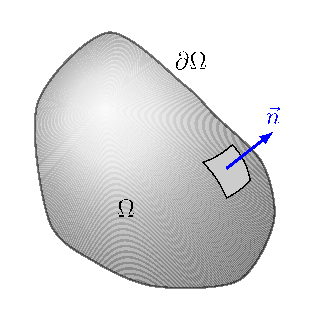
\includegraphics[scale=1]{Imagenes/Funcion_Green_01.eps}
\caption{Consideremos la ecuación de Poisson dentro de una región $\Omega$ acotada por una superficie $\partial \Omega$}
\label{fig:figura_07_01}
\end{figure}
\end{frame}

\begin{frame}
\frametitle{Ecuación no homogénea}
Esta es la forma no homogénea de la ecuación de Laplace.
\\
\bigskip
\pause
El término no homogéneo, $f (\vb{r})$, podría representar una fuente de calor en un problema de estado estacionario o una distribución de carga (fuente) en un problema electrostático.
\end{frame}

\begin{frame}
\frametitle{Considerando la fuente}
Ahora pensemos en la fuente como una fuente puntual en la que estamos interesados en la respuesta del sistema a esta fuente puntual.
\\
\bigskip
\pause
Si la fuente puntual está ubicada en un punto $\vb{\pderivada{r}}$, entonces la respuesta a la fuente puntual podría sentirse en los puntos $\vb{r}$.
\end{frame}

\begin{frame}
\frametitle{Estableciendo un nombre}
Llamaremos a esta respuesta $G(\vb{r}, \vb{\pderivada{r}})$. \pause La función de respuesta satisfacería una ecuación de fuente puntual de la forma:
\pause
\begin{align*}
\laplacian G(\vb{r}, \vb{\pderivada{r}}) = \delta (\vb{r} - \vb{\pderivada{r}})
\end{align*}
donde $\delta (\vb{r} - \vb{\pderivada{r}})$ es la función delta de Dirac.
\end{frame}

\begin{frame}
\frametitle{Propiedad de filtro de $\delta (r)$}
Una propiedad clave de esta función generalizada es la propiedad de filtro:
\pause
\begin{align*}
\scaleint{6ex}_{\bs \Omega} \delta (\vb{r} - \vb{\pderivada{r}}) \, f (\vb{r}) \dd{V} = f (\vb{\pderivada{r}})
\end{align*}
\end{frame}

\begin{frame}
\frametitle{Relación entre la función de Green y la solución}
La conexión entre la función de Green y la solución a la ecuación de Poisson se encuentra en la segunda identidad de Green:
\pause
\begin{align*}
\scaleint{6ex}_{\bs \partial \Omega} \bigg[ \phi \, \grad{\psi} - \psi \, \grad{\phi} \bigg] \cdot \vb{n} \dd{S} = \scaleint{6ex}_{\bs \Omega} \bigg[ \phi \, \laplacian{\psi} - \psi \, \laplacian{\phi} \bigg] \dd{V}
\end{align*}
\end{frame}

\begin{frame}
\frametitle{Usando la identidad}
Haciendo que $\phi = u (\vb{r})$ y $\psi = G (\vb{r}, \vb{\pderivada{r}})$, \pause considera que a continuación las integrales de volumen y de superficie, así como la diferenciación usando el operador $\grad$ se realizan usando las $\vb{r}$-coordenadas.
\end{frame}

\begin{frame}
\frametitle{Usando la identidad}
Se tiene que:
\begin{eqnarray}
\begin{aligned}[b]
&\scaleint{6ex}_{\bs \partial \Omega} \bigg[ u (\vb{r}) \, \grad{G (\vb{r}, \vb{\pderivada{r}})} - G (\vb{r}, \vb{\pderivada{r}}) \, \grad{u (\vb{r})} \bigg] \cdot \vb{n} \dd{S} = \\[0.5em] \pause
&= \scaleint{6ex}_{\bs \Omega} \bigg[ u (\vb{r}) \, \laplacian{G (\vb{r}, \vb{\pderivada{r}})} - G (\vb{r}, \vb{\pderivada{r}}) \, \laplacian{u (\vb{r})} \bigg] \dd{V} = \\[0.5em] \pause
&= \scaleint{6ex}_{\bs \Omega} \bigg[ u (\vb{r}) \, \delta (\vb{r} - \vb{\pderivada{r}}) - G (\vb{r}, \vb{\pderivada{r}}) \, f (\vb{r}) \bigg] \dd{V} = \\[0.5em] \pause
&= u (\vb{\pderivada{r}}) - \scaleint{6ex}_{\bs \Omega} G (\vb{r}, \vb{\pderivada{r}}) \, f (\vb{r}) \dd{V}
\end{aligned}
\label{eq:ecuacion_07_02}
\end{eqnarray}
\end{frame}

\begin{frame}
\frametitle{Resolviendo la expresión}
Al resolver para $u (\vb{\pderivada{r}})$, se tiene que:
\pause
\begin{eqnarray}
\begin{aligned}[b]
&u (\vb{\pderivada{r}}) = \scaleint{6ex}_{\bs \Omega} G (\vb{r}, \vb{\pderivada{r}}) \, f (\vb{r}) \dd{V} + \\[0.5em] \pause
&+ \scaleint{6ex}_{\bs \partial \Omega} \bigg[ u (\vb{r}) \, \grad{G (\vb{r}, \vb{\pderivada{r}})} - G (\vb{r}, \vb{\pderivada{r}}) \, \grad{u (\vb{r})} \bigg] \cdot \vb{n} \dd{S}
\end{aligned}
\label{eq:ecuacion_07_03}
\end{eqnarray}
\end{frame}

\begin{frame}
\frametitle{Ocupando las condiciones del problema}
Si tanto $u (\vb{r})$ como $G (\vb{r}, \vb{\pderivada{r}})$ satisfacen las condiciones de Dirichlet, $u = 0$ en $\partial \Omega$, \pause entonces la última integral se anula y nos queda:
\begin{align*}
u (\vb{\pderivada{r}}) = \scaleint{6ex}_{\bs \Omega} G (\vb{r}, \vb{\pderivada{r}}) \, f (\vb{r}) \dd{V}
\end{align*}
\end{frame}

\begin{frame}
\frametitle{Casos con simetría}
En algunas aplicaciones se presenta la simetría:
\pause
\begin{align*}
G (\vb{r}, \vb{\pderivada{r}}) = G (\vb{\pderivada{r}}, \vb{r})
\end{align*}
\pause
Por lo que el resultado se puede escribir como:
\pause
\begin{align*}
u (\vb{\pderivada{r}}) = \scaleint{6ex}_{\bs \Omega} G (\vb{r}, \vb{\pderivada{r}}) \, f (\vb{\pderivada{r}}) \dd{\pderivada{V}}
\end{align*}
\end{frame}

\begin{frame}
\frametitle{Resultado importante}
Entonces, si conocemos la función de Green, \pause \textocolor{red}{podemos resolver la ecuación diferencial no homogénea}.
\\
\bigskip
\pause
De hecho, podemos usar la función de Green para resolver problemas de valor límite y valor inicial no homogéneos.
\end{frame}

\section{Funciones de Green para valores iniciales}
\frame[allowframebreaks]{\tableofcontents[currentsection, hideothersubsections]}
\subsection{Planteamiento}

\begin{frame}
\frametitle{Tipo de problemas a resolver}
En esta parte revisaremos la solución de problemas con valores iniciales que involucran ED no homogéneas utilizando las funciones de Green.
\end{frame}

\begin{frame}
\frametitle{Tipo de ED}
Nuestro objetivo es resolver la ecuación diferencial no homogénea:
\pause
\begin{align}
a (t) \, \sderivada{y} (t) + b (t) \, \pderivada{y} (t) + c (t) \, y (t) = f (t)
\label{eq:ecuacion_07_04}
\end{align}
\pause
sujeta a las condiciones iniciales (CI):
\pause
\begin{align*}
y (0) = y_{0} \hspace{1cm} \pderivada{y} (0) = v_{0}
\end{align*}
\end{frame}

\begin{frame}
\frametitle{Reasignado la variable independiente}
Como estamos interesados en problemas de valor inicial, denotaremos la variable independiente como una variable temporal: $t$.
\\
\bigskip
\pause
La ec. (\ref{eq:ecuacion_07_04}) se puede escribir de forma compacta como:
\pause
\begin{align*}
L [y] = f
\end{align*}
\pause
donde $L$ es el operador diferencial:
\begin{align*}
L = a (t) \, \dv[2]{t} + b (t) \, \dv{t} + c (t) 
\end{align*}
\end{frame}

\begin{frame}
\frametitle{Solución al problema}
Cuya solución está dada por:
\pause
\begin{align*}
y = L^{-1} [f]
\end{align*}
\end{frame}

\begin{frame}
\frametitle{El inverso del operador}
El inverso de un operador diferencial es un operador integral, que buscamos escribir en la forma:
\pause
\begin{align*}
y (t) = \scaleint{6ex} G (t, \tau) \, f(\tau) \dd{\tau}
\end{align*}
\pause
La función $G (t, \tau)$ se conoce como el  \textocolor{ao}{kernel} (núcleo) del operador integral y  se denomina \textocolor{carmine}{función de Green}.
\end{frame}

\begin{frame}
\frametitle{Apoyo del curso de EDO1}
Tomando del curso de Ecuaciones Diferenciales I la parte de solución con el \textocolor{armygreen}{método de variación de parámetros}, \pause recordemos que este método es un procedimiento útil para la obtención de una solución particular $y_{p} (x)$ de la EDO lineal (no homogénea) y se basa en el conocimiento de la solución general de la lineal homogénea asociada a dicha EDO lineal.
\end{frame}

\begin{frame}
\frametitle{Seguimos entonces}
Hacemos que:
\pause
\begin{align}
y_{p} (t) = c_{1} (t) \, y_{1} (t) + c_{2} (t) \, y_{2} (t)
\label{eq:ecuacion_07_05}
\end{align}
\end{frame}

\begin{frame}
\frametitle{Sistema por resolver}
Encontramos que tenemos que resolver el sistema de ecuaciones:
\pause
\begin{eqnarray}
\begin{aligned}[b]
\pderivada{c}_{1} (t) \, y_{1} (t) + \pderivada{c}_{2} (t) \, y_{2} (t) &= 0 \\[0.5em] \pause
\pderivada{c}_{1} (t) \, \pderivada{y}_{1} (t) + \pderivada{c}_{2} (t) \, \pderivada{y}_{2} (t) &= \dfrac{f (t)}{q (t)}
\end{aligned}
\label{eq:ecuacion_07_06}
\end{eqnarray}
\end{frame}

\begin{frame}
\frametitle{Resolviendo el sistema}
Este sistema se resuelve fácilmente, para obtener entonces:
\pause
\begin{eqnarray}
\begin{aligned}[b]
\pderivada{c}_{1} (t) &= - \dfrac{f (t) \, y_{2} (t)}{a (t) \big[ y_{1} (t) \, \pderivada{y}_{2} (t)  - \pderivada{y}_{1} (t) \, y_{2} (t) \big]} \\[0.5em] \pause
\pderivada{c}_{2} (t) &= \dfrac{f (t) \, y_{1} (t)}{a (t) \big[ y_{1} (t) \, \pderivada{y}_{2} (t)  - \pderivada{y}_{1} (t) \, y_{2} (t) \big]}
\end{aligned}
\label{eq:ecuacion_07_07}
\end{eqnarray}
\end{frame}

\begin{frame}
\frametitle{Usando el Wronskiano}
Notemos que el denominador en estas expresiones involucra el Wronskiano de las soluciones al problema homogéneo, el cual viene dado por el determinante:
\pause
\begin{align*}
W (y_{1}, y_{2}) (t) = \mqty|
y_{1} (t) & y_{2} (t) \\
\pderivada{y}_{1} (t) & \pderivada{y}_{2} (t) |
\end{align*}
\end{frame}

\begin{frame}
\frametitle{Soluciones linealmente independientes}
Cuando $y_{1} (t)$ y $y_{2} (t)$ son linealmente independientes, \pause entonces el Wronskiano no es cero y tenemos garantizada una solución para el sistema anterior.
\end{frame}

\begin{frame}
\frametitle{Integrando el sistema}
Entonces, después de una integración, encontramos los parámetros como:
\pause
\begin{eqnarray}
\begin{aligned}
c_{1} (t) &= - \scaleint{6ex}_{\bs t_{0}}^{t} \dfrac{f (\tau) \, y_{2} (\tau)}{a (\tau) \, W (\tau)} \dd{\tau} \\[0.5em] \pause
c_{2} (t) &= \scaleint{6ex}_{\bs t_{1}}^{t} \dfrac{f (\tau) \, y_{1} (\tau)}{a (\tau) \, W (\tau)} \dd{\tau}
\end{aligned}
\label{eq:ecuacion_07_08}
\end{eqnarray}
donde $t_{0}$ y $t_{1}$ son constantes arbitrarias que se determinarán a partir de las condiciones iniciales.
\end{frame}

\begin{frame}
\frametitle{Solución particular}
Por lo tanto, la solución particular de la ec. (\ref{eq:ecuacion_07_04}) se puede escribir como:
\pause
\begin{eqnarray}
\begin{aligned}
y_{p} (t) &= y_{2} (t) \scaleint{6ex}_{\bs t_{1}}^{t} \dfrac{f (\tau) \, y_{1} (\tau)}{a (\tau) \, W (\tau)} \dd{\tau} + \\[0.5em] 
&- y_{1} (t) \scaleint{6ex}_{\bs t_{0}}^{t} \dfrac{f (\tau) \, y_{2} (\tau)}{a (\tau) \, W (\tau)} \dd{\tau}
\end{aligned}
\label{eq:ecuacion_07_09}
\end{eqnarray}
\end{frame}

\begin{frame}
\frametitle{Obteniendo las soluciones}
Comenzamos con la solución particular de la ec. (\ref{eq:ecuacion_07_09}) de la ED no homogénea (\ref{eq:ecuacion_07_04}).
\end{frame}

\begin{frame}
\frametitle{Obteniendo las soluciones}Esta se puede combinar con la solución general del problema homogéneo para dar la solución general de la ED no homogénea:
\begin{eqnarray}
\begin{aligned}
y_{p} (t) &= c_{1} y_{1} (t) + c_{2} y_{2} (t) +  y_{2} (t) \scaleint{6ex}_{\bs t_{1}}^{t} \dfrac{f (\tau) \, y_{1} (\tau)}{a (\tau) \, W (\tau)} \dd{\tau} + \\[0.5em] 
&- y_{1} (t) \scaleint{6ex}_{\bs t_{0}}^{t} \dfrac{f (\tau) \, y_{2} (\tau)}{a (\tau) \, W (\tau)} \dd{\tau}
\label{eq:ecuacion_07_10}
\end{aligned}
\end{eqnarray}
\end{frame}

\begin{frame}
\frametitle{Elección oportuna}
Sin embargo, se puede encontrar una elección adecuada de $t_{0}$ y $t_{1}$ para que no necesitemos escribir explícitamente la solución al problema homogéneo, $c_{1} y_{1} (t) + c_{2} y_{2} (t)$. 
\\
\bigskip
\pause
No obstante, configurar la solución de esta forma nos permitirá usar $t_{0}$ y $t_{1}$ para determinar soluciones particulares que satisfagan ciertas condiciones homogéneas.
\end{frame}

\begin{frame}
\frametitle{Usando la función de Green}
En particular, mostraremos que la ec. (\ref{eq:ecuacion_07_10}) se puede escribir en la forma:
\pause
\begin{align}
y_{p} (t) = c_{1} y_{1} (t) + c_{2} y_{2} (t) +  y_{2} (t) \scaleint{6ex}_{\bs 0}^{t} G (t,\tau) \, f (\tau) \dd{\tau}
\label{eq:ecuacion_07_11}
\end{align}
donde la función $G (t, \tau)$ será identificada como la función de Green.
\end{frame}

\begin{frame}
\frametitle{Tipos de problemas}
El objetivo es entonces desarrollar la técnica de la función de Green para resolver el problema de valor inicial:
\pause
\begin{eqnarray}
\begin{aligned}
a (t) \, \sderivada{y} (t) + b (t) \, &\pderivada{y} (t) + c (t) y(t) = f (t) \\[0.5em]
y (0) = y_{0}, \hspace{0.2cm} &\pderivada{y} (0) = v_{0}
\end{aligned}
\label{eq:ecuacion_07_12}
\end{eqnarray}
\end{frame}

\begin{frame}
\frametitle{Revisando el tipo de problemas}
Primero observamos que podemos resolver este problema de valores iniciales resolviendo dos problemas de valores iniciales separados.
\\
\bigskip
\pause
Suponemos que la solución del problema homogéneo satisface las condiciones iniciales originales:
\pause
\begin{eqnarray}
\begin{aligned}
a (t) \, \sderivada{y}_{h} (t) &+ b (t) \, \pderivada{y}_{h} (t) + c (t) y_{h} (t) = f (t) \\
y_{h} (0) = y_{0}, \hspace{0.2cm} &\pderivada{y}_{h} (0) = v_{0}
\end{aligned}
\label{eq:ecuacion_07_13}
\end{eqnarray}

\end{frame}

\begin{frame}
\frametitle{Solución particular}
Entonces asumimos que la solución particular satisface el problema:
\pause
\begin{align}
a (t) \, \sderivada{y}_{p} (t) + b (t) \, \pderivada{y}_{p} (t) + c (t) y_{h} (t) = f (t) \hspace{0.6cm} y_{p} (0) = y_{0}, \hspace{0.2cm} \pderivada{y}_{p} (0) = v_{0}
\label{eq:ecuacion_07_14}
\end{align}
\end{frame}

\begin{frame}
\frametitle{Aprovechando la linealidad}
Dado que la ecuación diferencial es lineal, se sabe que:
\pause
\begin{align*}
y (t) = y_{h} (t) + y_{p} (t)
\end{align*}
es una solución a la ecuación no homogénea.
\end{frame}

\begin{frame}
\frametitle{Solución que satisface las CI}
También, esta solución satisface las condiciones iniciales:
\pause
\begin{align*}
y (0) &= y_{h} (0) + y_{p} (0) = y_{0} + 0 = y_{0} \\[0.5em]
\pderivada{y} (0) &= \pderivada{y}_{h} (0) + \pderivada{y}_{p} (0) = v_{0} + 0 = v_{0}
\end{align*}
\end{frame}

\begin{frame}
\frametitle{Solución que cumpla las CI}
Por lo tanto, solo debemos centrarnos en encontrar una solución particular que satisfaga las condiciones iniciales homogéneas.
\\
\bigskip
\pause
Esto se hará encontrando valores para $t_{0}$ y $t_{1}$ en la ec. (\ref{eq:ecuacion_07_09}) que satisfagan las condiciones iniciales homogéneas: $y_{p} (0) = 0$ y $\pderivada{y}_{p} (0) = 0$
\end{frame}
% \par
% Primero, consideramos $y_{p} (0) = 0$. Tenemos que:
% \begin{align}
% y_{p} (0) = y_{2} (0) \scaleint{6ex}_{\bs t_{1}}^{0} \dfrac{f (\tau) \, y_{1} (\tau)}{a (\tau) \, W (\tau)} \dd{\tau} - y_{1} (0) \scaleint{6ex}_{\bs t_{0}}^{t} \dfrac{f (\tau) \, y_{2} (\tau)}{a (\tau) \, W (\tau)} \dd{\tau}
% \label{eq:ecuacion_07_15}
% \end{align}
% Aquí, $y_{1} (t)$ y $y_{2} (t)$ se toman como cualquier solución de la ecuación diferencial homogénea. Supongamos que $y_{1} (0) = 0$ y $y_{2} (0) \neq 0$. Entonces, tenemos:
% \begin{align}
% y_{p} (0) = y_{2} (0) \scaleint{6ex}_{\bs t_{1}}^{0} \dfrac{f (\tau) \, y_{1} (\tau)}{a (\tau) \, W (\tau)} \dd{\tau}
% \label{eq:ecuacion_07_16}
% \end{align}
% Podemos forzar que $y_{p} (0) = 0$ si hacemos que $t_{1} = 0$.
% \par
% Ahora, consideramos $\pderivada{y}_{p} (0) = 0$. Primero derivamos la solución y encontramos que:
% \begin{align}
% \pderivada{y}_{p} (t) = \pderivada{y}_{2} (t) \scaleint{6ex}_{\bs 0}^{t} \dfrac{f (\tau) \, y_{1} (\tau)}{a (\tau) \, W (\tau)} \dd{\tau} - \pderivada{y}_{1} (t) \scaleint{6ex}_{\bs t_{0}}^{t} \dfrac{f (\tau) \, y_{2} (\tau)}{a (\tau) \, W (\tau)} \dd{\tau}
% \label{eq:ecuacion_07_17}
% \end{align}
% ya que las contribuciones al diferenciar las integrales se cancelarán. Evaluando este resultado en $t = 0$, tenemos:
% \begin{align}
% \pderivada{y}_{p} (0) = - \pderivada{y}_{1} (0) \scaleint{6ex}_{\bs t_{0}}^{0} \dfrac{f (\tau) \, y_{2} (\tau)}{a (\tau) \, W (\tau)} \dd{\tau}
% \label{eq:ecuacion_07_18}
% \end{align}
% Suponiendo que $\pderivada{y}_{p} (0) \neq 0$, podemos hacer que $t_{0} = 0$.
% \par
% Entonces, hemos encontrado que:
% \begin{align}
% \begin{aligned}[b]
% y_{p} (x) &= y_{2} (t) \scaleint{6ex}_{\bs 0}^{t} \dfrac{f (\tau) \, y_{1} (\tau)}{a (\tau) \, W (\tau)} \dd{\tau} - y_{1} (t) \scaleint{6ex}_{\bs t_{0}}^{t} \dfrac{f (\tau) \, y_{2} (\tau)}{a (\tau) \, W (\tau)} \dd{\tau} = \\[0.5em]
% &= \scaleint{6ex}_{\bs 0}^{t} \bigg[ \dfrac{y_{1} (\tau) \, y_{2} (t) - y_{1} (t) \, y_{2} (\tau)}{a (\tau) \, W (\tau)} \bigg] \, f (\tau) \dd{\tau}
% \end{aligned}
% \label{eq:ecuacion_07_19}
% \end{align}
% Este resultado está en la forma correcta y podemos identificar el valor temporal o inicial: la función de Green. Entonces, la solución particular se da como:
% \begin{align}
% y_{p} (t) = \scaleint{6ex}_{\bs 0}^{t} G (t, \tau) \, f (\tau) \dd{\tau}
% \label{eq:ecuacion_07_20}
% \end{align}
% donde la condición inicial de la función de Green está definida como:
% \begin{align*}
% G (t, \tau) = \dfrac{y_{1} (\tau) \, y_{2} (t) - y_{1} (t) \, y_{2} (\tau)}{a (\tau) \, W (\tau)}
% \end{align*}

% A modo de resumen:
% \begin{tcolorbox}[title={\centering Solución para problema de valores iniciales con la función de Green}]

% La solución al problema de valores iniciales:
% \begin{align*}
% a (t) \, \sderivada{y} (t) + b (t) \pderivada{y} (t) + c (t) \, y (t) = f (t) \hspace{0.6cm} y (0) = y_{0}, \hspace{0.2cm} \pderivada{y} (0) = v_{0}
% \end{align*}
% es de la forma:
% \begin{align}
% y (t) = y_{h} (t) + \scaleint{6ex}_{\bs 0}^{t} G (t, \tau) \, f (t) \dd{\tau}
% \label{eq:ecuacion_07_21}
% \end{align}
% donde:
% \begin{align}
% G (t, \tau) = \dfrac{y_{1} (\tau) \, y_{2} (t) - y_{1} (t) \, y_{2} (\tau)}{a (\tau) \, W (\tau)}
% \label{eq:ecuacion_07_22}
% \end{align}
% es la función de Green, $y_{1}$, $y_{2}$, $y_{h}$ son soluciones de la ecuación homogénea que satisfacen:
% \begin{align*}
% y_{1} (0) = 0, \hspace{0.2cm} y_{2} (0) \neq 0, \hspace{0.2cm} \pderivada{y}_{1} (0) \neq 0, \hspace{0.2cm} \pderivada{y}_{2} (0) = 0, \hspace{0.2cm} y_{h} (0) = y_{0}, \hspace{0.2cm} \pderivada{y}_{h} (0) = v_{0}
% \end{align*}
% \end{tcolorbox}
% \begin{ejemplo}
% Resolvamos el problema del oscilador forzado:
% \begin{align*}
% \sderivada{x} + x = 2 \, \cos t, \hspace{0.5cm} x (0) = 4, \hspace{0.2cm} \pderivada{x} (0) = 0
% \end{align*}
% Primero resolvemos el problema homogéneo con las condiciones iniciales no homogéneas:
% \begin{align*}
% \sderivada{x}_{h} + x_{h} = 0, \hspace{0.5cm} x_{h} (0) = 4, \hspace{0.2cm} \pderivada{x}_{h} (0) = 0
% \end{align*}
% Cuya solución se obtiene fácilmente: $x_{h} (t) = 4 \, \cos t$, que se presenta en la figura (\ref{fig:figura_01}).
% \par
% A continuación, construimos la función de Green. Necesitamos dos soluciones linealmente independientes, $y_{1} (x)$, $y_{2} (x)$, para la ecuación diferencial homogénea que satisfaga diferentes condiciones homogéneas, $y_{1} (0) = 0$ y $\pderivada{y}_{2} (0) = 0$. Las soluciones más simples son $y_{1} (t) = \sen t$ y $y_{2} (t) = \cos t$.
% \par
% El Wronskiano para este ejemplo es:
% \begin{align*}
% W (t) = y_{1} (t) \, \pderivada{y}_{2} (t) - \pderivada{y}_{1} (t) \, y_{2} (t) = - \sin^{2} (t) - \cos^{2} (t) = - 1 
% \end{align*}
% Dado que en este ejercicio $a (t) = 1$, es posible calcular la función de Green:
% \begin{align}
% \begin{aligned}[b]
% G (t, \tau) &= G (t, \tau) = \dfrac{y_{1} (\tau) \, y_{2} (t) - y_{1} (t) \, y_{2} (\tau)}{a (\tau) \, W (\tau)} = \\[0.5em]
% &= \sin t \, \cos \tau - \sin \tau \, \cos t = \\[0.5em]
% &= \sin (t - \tau)
% \end{aligned}
% \label{eq:ecuacion_07_23}
% \end{align}
% Tomemos en cuenta que la función de Green depende de $t - \tau$. Si bien esto es útil en algunos contextos, usaremos la forma expandida al realizar la integración.
% \par
% Ahora podemos determinar la solución particular de la ecuación diferencial no homogénea. Tenemos que:
% \begin{align}
% \begin{aligned}[b]
% x_{p} (t) &= \scaleint{6ex}_{\bs 0}^{t} G (t, \tau) \, f (\tau) \dd{\tau} = \\[0.5em]
% &= \scaleint{6ex}_{\bs 0}^{t} (\sin t \, \cos \tau - \sin \tau \, \cos t) (2 \, \cos \tau) \dd{\tau} = \\[0.5em]
% &= 2 \sin t \, \scaleint{6ex}_{\bs 0}^{t} \cos^{2} \tau \dd{\tau} - 2 \cos t \, \scaleint{6ex}_{\bs 0}^{t} \sin \tau \, \cos \tau \dd{\tau} = \\[0.5em]
% &= 2 \sin t \, \bigg[ \dfrac{\tau}{2} + \dfrac{1}{2} \, \sin 2 \tau \bigg] \eval_{0}^{t} - 2 \cos t \, \bigg[ \dfrac{1}{2} \, \sin^{2} \tau \bigg] \eval_{0}^{t} = \\[0.5em]
% &= t \, \sin t
% \end{aligned}
% \label{eq:ecuacion_07_24}
% \end{align}

% En la figura (\ref{fig:figura_01}) se muestran las soluciones al caso homogéneo como no homogéneo.
% \begin{figure}[H]
%     \centering
%     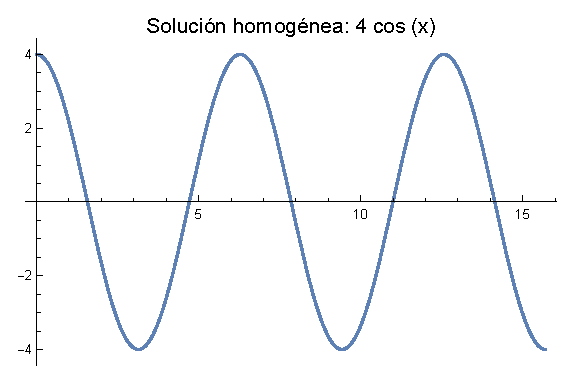
\includegraphics[scale=1]{Imagenes/Plot_Oscilador_Forzado_Green_01.eps}
%     \caption{Soluciones a la EDO en el caso homogéneo y no homogéneo.}
%     \label{fig:figura_01}
% \end{figure}

% Por lo tanto, la solución al problema no homogéneo, es la suma es la solución del problema homogéneo y esta solución particular:
% \begin{align*}
% x (t) = 4 \, \cos t + t \, \sin t
% \end{align*}
% La gráfica de la solución se muestra en la figura (\ref{fig:figura_02}):
% \begin{figure}[H]
%     \centering
%     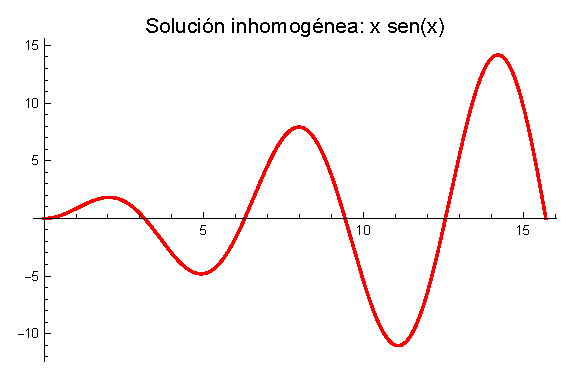
\includegraphics[scale=1]{Imagenes/Plot_Oscilador_Forzado_Green_02.eps}
%     \caption{Solución completa a la EDO no homogénea.}
%     \label{fig:figura_02}
% \end{figure}

% \end{ejemplo}

% \section{Valores de frontera y funciones de Green.}

% En el numeral anterior, resolvimos problemas de valores iniciales no homogéneos usando una función de Green. En esta sección extenderemos este método a la solución de problemas de valores en la frontera no homogéneos usando una función de Green. Recordemos que el objetivo es resolver la ecuación diferencial no homogénea:
% \begin{align*}
% L [y] = f, \hspace{0.6cm} a \leq x \leq b
% \end{align*}
% donde $L$ es un operador diferencial y $y (x)$ satisface las condiciones de frontera en $x = a$ y $x = b$. La solución viene dada formalmente por:
% \begin{align*}
% y = L^{-1} [y]
% \end{align*}

% El \emph{inverso de un operador diferencial es un operador integral}, que buscamos escribir de la forma:
% \begin{align*}
% y (x) = \scaleint{6ex}_{a}^{b} G (x, \xi) \, f (\xi) \dd{\xi} 
% \end{align*}
% La función $G (x, \xi)$ se conoce como el \emph{kernel} (núcleo) del operador integral y se le llama \emph{función de Green}.
% \par
% Consideraremos problemas de valores en la frontera en forma de Sturm-Liouville\footnote{Este concepto será la parte central del contenido del Tema 3, que sin pérdida de generalidad, podemos mencionar en este momento.}:
% \begin{align}
% \dv{x} \bigg[ p (x) \, \dv{y (x)}{x} \bigg] + q (x) \, y (x) = f (x), \hspace{0.6cm} a < x < b
% \label{eq:ecuacion_07_25}
% \end{align}
% con valores fijos de $y (x)$ en la frontera, $y (a) = 0$ y $y (b) = 0$. Sin embargo, la teoría general funciona para otras formas de condiciones de frontera homogéneas.
% \par
% Buscamos la función de Green resolviendo primero la ecuación diferencial no homogénea usando el método de variación de parámetros. Suponemos una solución particular de la forma
% \begin{align*}
% y_{p} (x) = c_{1} (x) \, y_{1} (x) + c_{2} (x) \, y_{2} (x)
% \end{align*}
% que se forma a partir de dos soluciones linealmente independientes del problema homogéneo, $y_{i} (x), i = 1, 2$. Habíamos encontrado que las funciones de los coeficientes satisfacen las ecuaciones:
% \begin{align}
% \begin{aligned}[b]
% \pderivada{c}_{1} (t) \, y_{1} (t) + \pderivada{c}_{2} (t) \, y_{2} (t) &= 0 \\[0.5em]
% \pderivada{c}_{1} (t) \, \pderivada{y}_{1} (t) + \pderivada{c}_{2} (t) \, \pderivada{y}_{2} (t) &= \dfrac{f (t)}{q (t)}
% \end{aligned}
% \label{eq:ecuacion_07_26}
% \end{align}
% resolviendo este sistema, se obtiene:
% \begin{align*}
% \pderivada{c}_{1} (x) &= - \dfrac{f \, y_{2}}{p \, W (y_{1}, y_{2})} \\[0.5em]
% \pderivada{c}_{2} (x) &= \dfrac{f \, y_{1}}{p \, W (y_{1}, y_{2})}
% \end{align*}
% donde $W (y_{1}, y_{2}) = y_{1} \, \pderivada{y}_{2} - \pderivada{y}_{1} \, y_{2}$ es el Wronskiano. Integrando las expresiones para sustituirlas de regreso en la solución particular, se encuentra que:
% \begin{align*}
% y (x) = y_{2} (x) \scaleint{6ex}_{\bs x_{1}}^{x_{2}} \dfrac{f (\xi) \, y_{1} (\xi)}{p (\xi) \, W (\xi)} \dd{\xi} - y_{1} (x) \scaleint{6ex}_{\bs x_{0}}^{x} \dfrac{f (\xi) \, y_{2} (\xi)}{p (\xi) \, W (\xi)} \dd{\xi}
% \end{align*}
% donde $x_{0}$ y $x_{1}$ se determinarán utilizando las condiciones de frontera. En particular, buscaremos $x_{0}$ y $x_{1}$ para que la solución al problema de valores en la frontera pueda escribirse como una integral simple que involucre una función de Green. %Notemos que podemos absorber la solución del problema homogéneo, yh(x), en las integrales con una elección apropiada de límites en las integrales.
% \par
% Ahora buscamos satisfacer las condiciones $y (a) = 0$ y $y (b) = 0$. Primero usamos soluciones de la ecuación diferencial homogénea que satisfacen $y_{1} (a) = 0$, $y_{2} (b) = 0$ y $y_{1} (b) \neq 0$, $y_{2} (a) \neq 0$. Evaluando $y (x)$ en $x = 0$, tenemos que:
% \begin{align}
% \begin{aligned}[b]
% y (a) &= y_{2} (a) \scaleint{6ex}_{\bs x_{1}}^{a} \dfrac{f (\xi) \, y_{1} (\xi)}{p (\xi) \, W (\xi)} \dd{\xi} - y_{1} (a) \scaleint{6ex}_{\bs x_{0}}^{a} \dfrac{f (\xi) \, y_{2} (\xi)}{p (\xi) \, W (\xi)} \dd{\xi} = \\[0.5em]
% &= y_{2} (a) \scaleint{6ex}_{\bs x_{1}}^{a} \dfrac{f (\xi) \, y_{1} (\xi)}{p (\xi) \, W (\xi)} \dd{\xi}
% \end{aligned}
% \label{eq:ecuacion_07_27}
% \end{align}
% Podemos satisfacer la condición en $x = a$ si escogemos $x_{1} = a$. De manera similar, en $x = b$, encontramos que:
% \begin{align}
% \begin{aligned}[b]
% y (b) &= y_{2} (b) \scaleint{6ex}_{\bs x_{1}}^{b} \dfrac{f (\xi) \, y_{1} (\xi)}{p (\xi) \, W (\xi)} \dd{\xi} - y_{1} (b) \scaleint{6ex}_{\bs x_{0}}^{b} \dfrac{f (\xi) \, y_{2} (\xi)}{p (\xi) \, W (\xi)} \dd{\xi} = \\[0.5em]
% &= - y_{1} (b) \scaleint{6ex}_{\bs x_{0}}^{b} \dfrac{f (\xi) \, y_{2} (\xi)}{p (\xi) \, W (\xi)} \dd{\xi}
% \end{aligned}
% \label{eq:ecuacion_07_28}
% \end{align}
% Esta expresión se anula para $x_{0} = b$.

% Así, hemos encontrado que la solución es de la forma:
% \begin{align}
% y (x) &= y_{2} (x) \scaleint{6ex}_{\bs a}^{x} \dfrac{f (\xi) \, y_{1} (\xi)}{p (\xi) \, W (\xi)} \dd{\xi} - y_{1} (x) \scaleint{6ex}_{\bs b}^{x} \dfrac{f (\xi) \, y_{2} (\xi)}{p (\xi) \, W (\xi)} \dd{\xi}
% \label{eq:ecuacion_07_29}
% \end{align}
% Esta solución se puede escribir en forma compacta tal como lo hicimos para el problema de valores iniciales del numeral anterior. Buscamos una función de Green para que la solución se pueda escribir como una sola integral. Podemos mover las funciones de $x$ debajo de la integral. Además, dado que $a < x < b$, podemos invertir los límites en la segunda integral. Esto nos da:
% \begin{align}
% y (x) &= \scaleint{6ex}_{\bs x}^{a} \dfrac{f (\xi) \, y_{1} (\xi) \, y_{2} (x)}{p (\xi) \, W (\xi)} \dd{\xi} + \scaleint{6ex}_{\bs x}^{b} \dfrac{f (\xi) \, y_{1} (x) \, y_{2} (\xi)}{p (\xi) \, W (\xi)} \dd{\xi}
% \label{eq:ecuacion_07_30}
% \end{align}
% Este resultado se puede ahora escribir de una manera compacta:
% \begin{tcolorbox}[title={\centering Solución para problema de CDF con la función de Green}]

% La solución para el problema de condiciones de frontera:
% \begin{align}
% \begin{aligned}
% \dv{x} \bigg[ p (x) \, \dv{y (x)}{x} \bigg] &+ q (x) \, y (x) = f (x), \hspace{0.6cm} a < x < b \\[0.5em]
% &y (a) = 0, \hspace{0.4cm} y (b) = 0
% \end{aligned}
% \label{eq:ecuacion_07_31}
% \end{align}
% toma la forma:
% \begin{align}
% y (x) = \scaleint{6ex}_{\bs a}^{b} G (x, \xi) \, f (\xi) \dd{\xi}
% \label{eq:ecuacion_07_32}
% \end{align}
% donde la función de Green es una función en partes definida como:
% \begin{align}
% G (x, \xi) = \begin{cases}
% \dfrac{y_{1} (\xi) \, y_{2} (x)}{p \, W}, & a \leq \xi \leq x \\[0.5em]
% \dfrac{y_{1} (x) \, y_{2} (\xi)}{p \, W}, & x \leq \xi \leq b
% \end{cases}
% \label{eq:ecuacion_07_33}
% \end{align}
% donde $y_{1} (x)$ y $y_{2} (x)$ son soluciones al problema homogéneo que satisfacen $y_{1} (a) = 0$, $y_{2} (b) = 0$ y $y_{1} (b) \neq 0$, $y_{2} (a) \neq 0$.
% \end{tcolorbox}

% La función de Green satisface varias propiedades, que revisaremos más adelante. Por ejemplo, la función de Green satisface las condiciones de frontera en $x = a$ y $x = b$. Por lo tanto:
% \begin{align*}
% G (a, \xi) &= \dfrac{y_{1} (a) \, y_{2} (x)}{p \, W} = 0 \\[0.5em]        
% G (b, \xi) &= \dfrac{y_{1} (\xi) \, y_{2} (b)}{p \, W} = 0
% \end{align*}
% Además, la función de Green es simétrica en sus argumentos. Intercambiando los argumentos nos devuelve:
% \begin{align}
% G (\xi, x) = \begin{cases}
% \dfrac{y_{1} (x) \, y_{2} (\xi)}{p \, W}, & a \leq x \leq \xi \\[0.5em]
% \dfrac{y_{1} (\xi) \, y_{2} (x)}{p \, W}, & \xi \leq x \leq b
% \end{cases}
% \label{eq:ecuacion_07_34}
% \end{align}    
% Pero revisando de manera cuidadosa a la forma original, tenemos que:
% \begin{align*}
% G (x, \xi) = G (\xi, x)
% \end{align*}

% Haremos uso de estas propiedades más adelante para determinar rápidamente las funciones de Green para otros problemas de valores en la frontera.

% \begin{ejemplo}
% Usando la función de Green para CDF, resuelve el problema:
% \begin{align*}
% \sderivada{y} = x^{2}, \hspace{0.6cm} y (0) = 0 = y (1)
% \end{align*}
% Primero resolvemos la ecuación homogénea, $\sderivada{y} = 0$. Después de dos integraciones, tenemos que:
% \begin{align*}
% y (x) = A \, x + B
% \end{align*}
% donde falta determinar las constantes $A$ y $B$.
% \par
% Necesitamos una solución que satisfaga $y_{1} (0) = 0$. Por lo tanto:
% \begin{align*}
% 0 = y_{1} (0) = B
% \end{align*}

% \end{ejemplo}
% Entonces, podemos elegir $y_{1} (x) = x$, ya que $A$ es arbitrario.
% \par
% La otra solución tiene que satisfacer $y_{2} (1) = 0$. Entonces:
% \begin{align*}
% 0 = y_{2} (1) = A + B
% \end{align*}
% Esto se puede resolver para $B = - A$. Nuevamente, $A$ es arbitraria y elegimos $A = - 1$. Por tanto:
% \begin{align*}
% y_{2} (x) = 1 - x
% \end{align*}
% Las soluciones al problema homogéneo se presentan en la figura (\ref{fig:figura_03}).
% \begin{figure}[H]
%     \centering
%     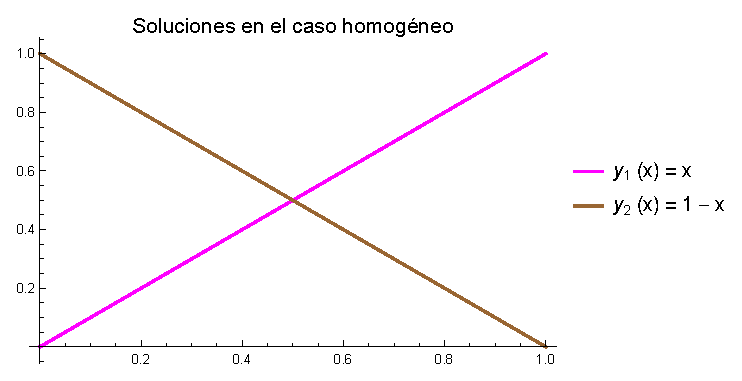
\includegraphics[scale=1]{Imagenes/Plot_EDONH_Green_01.eps}
%     \caption{Soluciones $y_{1} (x)$ y $y_{2} (x)$ para el caso de la ED homogénea.}
%     \label{fig:figura_03}
% \end{figure}

% Para este problema $p (x) = 1$. Así, para $y_{1} (x) = x$ y $y_{2} (x) = 1 - x$, el producto:
% \begin{align*}
% p (x) \, W (x) =  y_{1} (x) \, \pderivada{y}_{2} (x) - \pderivada{y}_{1} (x) \, y_{2} (x) = x (-1) -  1(1 - x) = - 1
% \end{align*}
% Tomemos en cuenta que $p (x) \, W (x)$ es una constante, como debería ser.
% \par
% Ahora construimos la función de Green. Así tenemos:
% \begin{align}
% G (x, \xi) = \begin{cases}
% - \xi \, (1 - x), & 0 \leq \xi \leq x \\
% - x \, (1 - \xi), & x \leq \xi \leq 1
% \end{cases}
% \label{eq:ecuacion_07_35}
% \end{align}

% Observemos la simetría entre las dos partes de la función de Green. \break \hfill Además, la función de Green satisface condiciones de frontera homogéneas: 
% \begin{align*}
% G (0, \xi) &= 0, \mbox{ de la parte inferior}, \\[0.5em]
% G (1, \xi) &= 0, \mbox{ de la parte superior}
% \end{align*}
% Finalmente, sustituimos la función de Green en la forma integral de la solución y evaluamos la integral:
% \begin{align}
% \begin{aligned}[b]
% y (x) &= \scaleint{6ex}_{0}^{1} G (x, \xi) \, f (\xi) \dd{\xi} = \\[0.5em]
% &= \scaleint{6ex}_{0}^{1} G (x, \xi) \, \xi^{2} \dd{\xi} = \\[0.5em]
% &= - \scaleint{6ex}_{0}^{x} \xi \, (1 - x) \, \xi^{2} \dd{\xi} - \scaleint{6ex}_{x}^{1} x \, (1 - \xi) \, \xi^{2} \dd{\xi} = \\[0.5em]
% &= - (1 - x) \scaleint{6ex}_{0}^{x} \xi^{3} \dd{\xi} - x \, \scaleint{6ex}_{x}^{1} (\xi^{2} - \xi^{3}) \dd{\xi} = \\[0.5em]
% &= - (1 - x) \bigg[ \dfrac{\xi^{4}}{4} \bigg] \eval_{0}^{4} - x \bigg[ \dfrac{\xi^{3}}{3} - \dfrac{\xi^{4}}{4} \bigg] \eval_{x}^{1} = \\[0.5em]
% &= \dfrac{1}{4} (1 - x) x^{4} - \dfrac{1}{12} \, x (4 - 3) + \dfrac{1}{12} \, x (4 x^{3} - 3 x^{4}) = \\[0.5em]
% &= \dfrac{1}{12} (x^{4} - x)
% \end{aligned}
% \label{eq:ecuacion_07_36}
% \end{align}
% Revisando la solución, se verifica fácilmente que la EDO
% \begin{align*}
% \sderivada{y} = x^{2}
% \end{align*}
% se satisface para las CDF $y (0) = 0$ y $y (1) = 0$. La solución completa al caso no homogéneo se presenta en la figura (\ref{fig:figura_04}).
% \begin{figure}[H]
%     \centering
%     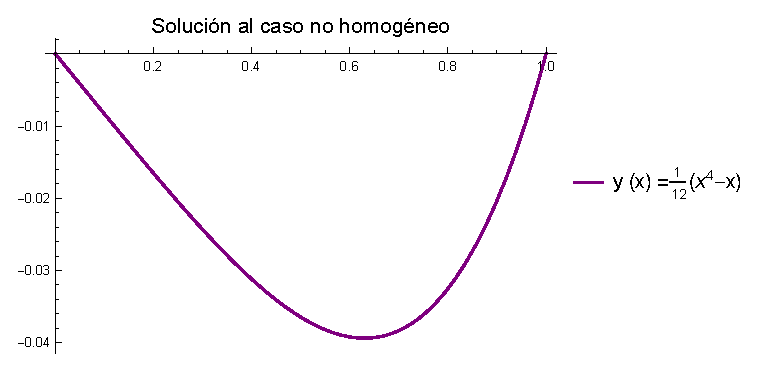
\includegraphics[scale=1]{Imagenes/Plot_EDONH_Green_02.eps}
%     \caption{Solución a la ED no homogénea que cumple con las CDF indicadas en el ejercicio.}
%     \label{fig:figura_04}
% \end{figure}

% \section{Propiedades de la función de Green.}

% Hemos mencionado algunas propiedades de las funciones de Green en el último numeral.
% \par
% En esta parte revisaremos algunas de estas propiedades como una herramienta para construir rápidamente funciones de Green para problemas de valores en la frontera. Enumeramos cinco propiedades básicas:
% \begin{enumerate}
% \item \textbf{Ecuación diferencial: } La función de Green con valor de frontera satisface la ecuación diferencial:
% \begin{align*}
% \pdv{x} \bigg[ p (x) \, \pdv{G (x, \xi)}{x} \bigg] + q (x) \, G (x, \xi) = 0, \hspace{0.5cm} x \neq \xi
% \end{align*}
% Esto se establece fácilmente. Para $x < \xi$ estamos en el  segundo caso y $G (x, \xi)$ es proporcional a $y_{1} (x)$. Así, dado que $y_{1} (x)$ es una solución de la ecuación homogénea, también lo es $G (x, \xi)$. Para $x > \xi$ estamos en el primer caso y $G (x, \xi)$ es proporcional a $y_{2} (x)$. Entonces, una vez más $G (x, \xi)$ es una solución del problema homogéneo.
% \item \textbf{Condiciones de frontera :} En el ejemplo del numeral anterior, se vio que $G (a, \xi) = 0$ y $G (b, \xi) = 0$. Por ejemplo, para $x = a$ estamos en el segundo caso y $G (x, \xi)$ es proporcional a $y_{1} (x)$. Por lo tanto, cualquier condición que satisfaga $y_{1} (x)$, $G (x, \xi)$ la satisfará. Se puede hacer una afirmación similar para $x = b$.
% \item \textbf{Simetría o reciprocidad :} $G (x, \xi) = G (\xi, x)$.
% \par
% \noindent
% Se demostró esta propiedad en el numeral anterior.
% \item \textbf{Continuidad de $\mathbf{G}$ en $x = \xi$ :} $G (\xi^{+}, \xi) = G (\xi^{-}, \xi)$
% \par
% \noindent
% Aquí definimos $\xi^{\pm}$ a través de los límites de una función cuando $x$ tiende a $\xi$ desde arriba o desde abajo En particular:
% \begin{align*}
% G (\xi^{+}, x) &= \lim_{x \uparrow \xi}, \hspace{0.4cm} x > \xi \\[0.5em]
% G (\xi^{-}, x) &= \lim_{x \downarrow \xi}, \hspace{0.4cm} x < \xi
% \end{align*}
% Haciendo $x = \xi$ en ambos casos, tenemos que:
% \begin{align*}
% \dfrac{y_{1} (\xi) \, y_{2} (\xi)}{p \, W} = \dfrac{y_{1} (\xi) \, y_{2} (\xi)}{p \, W}
% \end{align*}
% Por tanto, hemos establecido la continuidad de $G (x, \xi)$ entre los dos casos en $x = \xi$.
% \item \textbf{Salto de discontinuidad de $\displaystyle \pdv{G}{x}$ en $x = \xi$ :}
% \begin{align*}
% \pdv{G (\xi^{+}, \xi)}{x} - \pdv{G (\xi^{-}, \xi)}{x} = \dfrac{1}{p (\xi)}
% \end{align*}
% Esta propiedad no es tan obvia. Primero calculamos las derivadas observando qué caso está involucrado y luego evaluamos las derivadas y las restamos. Así, tenemos lo siguiente:
% \begin{align}
% \begin{aligned}[b]
% \pdv{G (\xi^{+}, \xi)}{x} - \pdv{G (\xi^{-}, \xi)}{x} &= - \dfrac{1}{p \, W} \, y_{1} (\xi) \, \pderivada{y}_{2} (\xi) + \dfrac{1}{p \, W} \, \pderivada{y}_{1} (\xi) \, y_{2} (\xi) = \\[0.5em]
% &= - \dfrac{\pderivada{y}_{1} (\xi) \, y_{2} (\xi) - y_{1} (\xi) \, \pderivada{y}_{2} (\xi)}{p (\xi) \, \big[ y_{1} (\xi) \, \pderivada{y}_{2} (\xi) - \pderivada{y}_{1} (\xi) \, y_{2} (\xi) \big]} = \\[0.5em]
% &= \dfrac{1}{p (\xi)}
% \end{aligned}
% \label{eq:ecuacion_07_37}
% \end{align}
% \end{enumerate}
% Se presenta un resumen de las propiedades de la función de Green con condiciones de frontera basado en la solución anterior.
% \begin{tcolorbox}[title={\centering Propiedades de la función de Green}]

% \begin{enumerate}
% \item \textbf{Ecuación diferencial:}
% \begin{align*}
% \pdv{x} \bigg[ p (x) \, \pdv{G (x, \xi)}{x} \bigg] + q (x) \, G (x, \xi) = 0, \hspace{0.5cm} x \neq \xi
% \end{align*}
% \item \textbf{Condiciones de frontera :} Con cualesquiera condiciones $y_{1} (x)$ y $y_{2} (x)$ que se satisfagan, $G (x, \xi)$ se satisface.
% \item \textbf{Simetría o reciprocidad :} $G (x, \xi) = G (\xi, x)$
% \item \textbf{Continuidad de $\mathbf{G}$ en $x = \xi$ :} $G (\xi^{+}, \xi) = G (\xi^{-}, \xi)$
% \item \textbf{Salto de discontinuidad de $\displaystyle \pdv{G}{x}$ en $x = \xi$ :}
% \begin{align*}
% \pdv{G (\xi^{+}, \xi)}{x} - \pdv{G (\xi^{-}, \xi)}{x} = \dfrac{1}{p (\xi)}
% \end{align*}
% \end{enumerate}
% \end{tcolorbox}
% Ahora mostramos cómo el conocimiento y manejo de estas propiedades, permite construir rápidamente una función de Green con un ejemplo.
% \begin{ejemplo}
% Construye la función de Green para el siguiente problema:
% \begin{align*}
% \sderivada{y} &+ \omega^{2} \, y = f(x) \hspace{0.6cm} 0 < x < 1 \\[0.5em]
% &=y (0) = 0 = y (1) \hspace{0.6cm} \omega \neq 0
% \end{align*}
% \begin{enumerate}
% \item \textbf{Encontrar las soluciones a la ecuación homogénea.}
% \par
% \noindent
% Una solución general a la ecuación homogénea está dada por:
% \begin{align*}
% y_{h} (x) = c_{1} \, \sin \omega x + c_{2} \, \cos \omega x
% \end{align*}
% Por lo que, para $x \neq \xi$:
% \begin{align*}
% G (x, \xi) = c_{1} (\xi) \, \sin \omega x + c_{2} (\xi) \, \cos \omega x
% \end{align*}
% \item \textbf{Condiciones de frontera.}
% \par
% \noindent
% Primero, tenemos que $G (0, \xi) = 0$ para $0 \leq x \leq \xi$. Así:
% \begin{align*}
% G (0, \xi) = c_{2} (\xi) \, \cos \omega x = 0
% \end{align*}
% Entonces:
% \begin{align*}
% G (x, \xi) = c_{1} (\xi) \, \sin \omega x = 0, \hspace{0.5cm} 0 \leq x \leq \xi
% \end{align*}
% Segundo, tenemos que $G (1, \xi) = 0$, para $\xi \leq x \leq 1$. Por lo tanto:
% \begin{align*}
% G (1, \xi) = c_{1} (\xi) \, \sin \omega + c_{2} (\xi) \, \cos \omega = 0
% \end{align*}
% Se puede elegir una solución haciendo que:
% \begin{align*}
% c_{2} (\xi) = - c_{1} (\xi) \, \tan \omega
% \end{align*}
% Esto nos proporciona:
% \begin{align*}
% G (x, \xi) = c_{1} (\xi) \, \sin \omega x - c_{1} (\xi) \, \tan \omega \, \cos \omega x
% \end{align*}
% Esto se puede simplificar factorizando el $c_{1} (\xi)$ y colocando los términos restantes sobre un denominador común. El resultado es:
% \begin{align}
% \begin{aligned}[b]
% G (x, \xi) &= \dfrac{c_{1} (\xi)}{\cos \omega} \big[ \sin \omega x \, \cos \omega - \sin \omega \, \cos \omega x \big] = \\[0.5em]
% &= - \dfrac{c_{1} (\xi)}{\cos \omega} \, \sin \omega (1 - x)
% \end{aligned}
% \label{eq:ecuaction_07_38}
% \end{align}
% Dado que el coeficiente es arbitrario en este punto, podemos escribir el resultado como:
% \begin{align*}
% G (x, \xi) = d_{1} (\xi) \, \sin \omega (1 - x), \hspace{0.5cm} \xi \leq x \leq 1
% \end{align*}
% Observamos que podríamos haber comenzado con $y_{2} (x) = \sin \omega (1 - x)$ como una de las soluciones linealmente independientes del problema homogéneo, anticipando que $y_{2} (x)$ satisface la segunda condición de frontera.
% \item \textbf{Simetría o reciprocidad.}
% \par
% \noindent
% Si imponemos que $G (x, \xi) = G (\xi, x)$. En este punto tenemos que:
% \begin{align*}
% G (x, \xi) = \begin{cases}
% c_{1} (\xi) \, \sin \omega x & 0 \leq x \leq \xi \\[0.5em]
% d_{1} (\xi) \, \sin \omega (1 - x) & \xi \leq x \leq 1
% \end{cases}
% \end{align*}
% Podemos hacer que los casos sean simétricos eligiendo las formas correctas para $c_{1} (\xi)$ y $d_{1} (\xi)$. Elegimos :
% \begin{align*}
% c_{1} (\xi) &= C \, \sin \omega (1 - \xi) \\[0.5em]
% d_{1} (\xi) &= C \, \sin \omega \xi
% \end{align*}
% Luego entonces:
% \begin{align*}
% G (x, \xi) = \begin{cases}
% c_{1} (\xi) \, \sin \omega x & 0 \leq x \leq \xi \\[0.5em]
% d_{1} (\xi) \, \sin \omega (1 - x) & \xi \leq x \leq 1
% \end{cases}
% \end{align*}
% Ahora la función de Green es simétrica y todavía tenemos que determinar la constante $C$. Notemos que podríamos haber llegado a este punto usando el resultado del método de variación de parámetros donde $C = \dfrac{1}{p \, W}$.
% \item \textbf{Continuidad de $G (x, \xi)$}.
% \par
% \noindent
% Ya tenemos continuidad en virtud de la simetría impuesta en el último paso.
% \item \textbf{Salto de discontinuidad de $\displaystyle \pdv{x} G (x \xi)$}
% \par
% \noindent
% Todavía necesitamos determinar $C$. Podemos hacer esto usando salto de discontinuidad en la derivada:
% \begin{align*}
% \pdv{G (\xi^{+}, \xi)}{x} - \pdv{G (\xi^{-}, \xi)}{x} = \dfrac{1}{p (\xi)}
% \end{align*}
% En este problema $p (x) = 1$. Sustituyendo la función de Green, se tiene que:
% \begin{align}
% \begin{aligned}[b]
% 1 & = \pdv{G (\xi^{+}, \xi)}{x} - \pdv{G (\xi^{-}, \xi)}{x} = \\[0.5em]
% &= \pdv{x} \big[ C \, \sin \omega (1 - x) \, \sin \omega \xi \big] \eval_{x = \xi} + \\[0.5em]
% &- \pdv{x} \big[ C \, \sin \omega (1 - \xi) \, \sin \omega \xi \big] \eval_{x = \xi} = \\[0.5em]
% &= - \omega \, C \, \cos \omega (1 - \xi) \, \sin \omega \xi - \omega \, C \, \sin \omega (1 - \xi) \, \cos \omega  \xi = \\[0.5em]
% &= - \omega \, C \, \sin \omega (\xi + 1 - \xi) = \\[0.5em]
% &= - \omega \, C \, \sin \omega
% \end{aligned}
% \label{eq:ecuacion_07_39}
% \end{align}
% \end{enumerate}
% Por lo tanto:
% \begin{align*}
% C = - \dfrac{1}{\omega \, \sin \omega}
% \end{align*}
% Finalmente, hemos obtenido la función de Green:
% \begin{align}
% G (x, \xi) = \begin{cases}
% - \dfrac{\sin \omega (1 - \xi) \, \sin \omega x}{\omega \, \sin \omega} & 0 \leq x \leq \xi \\[1em]
% - \dfrac{\sin \omega (1 - x) \, \sin \omega \xi}{\omega \, \sin \omega} & \xi \leq x \leq 1
% \end{cases}
% \label{eq:ecuacion_07_40}
% \end{align}
% \end{ejemplo}


\end{document}